\documentclass[11pt,oneside]{article}
\usepackage[a4paper,margin=26mm,headheight=15pt]{geometry}
\usepackage[T1]{fontenc}
\usepackage[utf8]{inputenc}
\IfFileExists{libertinus.sty}{\usepackage{libertinus}}{\usepackage{lmodern}}
\usepackage{microtype}
\usepackage{amsmath,amssymb,amsthm,mathtools,mathrsfs,bm}
\usepackage{booktabs,longtable,array,tabularx,multirow}
\usepackage{graphicx}
\usepackage{caption}
\usepackage{xcolor}
\usepackage{enumitem}
\usepackage{fancyhdr}
\usepackage{titlesec}
\usepackage{listings}
\usepackage{xurl}
\usepackage[hypertexnames=false]{hyperref}
\usepackage[nameinlink,noabbrev]{cleveref}

\graphicspath{
  {assets/rvachev_up_polynomial_representation/generated/}
}

\definecolor{linkblue}{RGB}{25,75,135}
\definecolor{deepgreen}{RGB}{28,103,76}
\definecolor{shadegray}{RGB}{246,247,249}
\definecolor{rulegray}{RGB}{195,201,208}
\hypersetup{
  colorlinks=true,
  linkcolor=linkblue,
  citecolor=deepgreen,
  urlcolor=linkblue,
  pdftitle={Exact Polynomial Synthesis from Rvachev Up-Atoms},
  pdfsubject={Finite exact representation of polynomials by shifted and scaled
    Rvachev up-functions: common-scale dictionaries, antiderivative-train
    windows, and minimal atom counts},
  pdfkeywords={Rvachev up function, Fabius function, Strang-Fix, polynomial
    reproduction, Thue-Morse, q-integer, binary partitions, Appell polynomials,
    shift-invariant space}
}

\pagestyle{fancy}
\fancyhf{}
\fancyhead[L]{\small Up-atom polynomial synthesis}
\fancyhead[R]{\small\nouppercase{\leftmark}}
\fancyfoot[C]{\thepage}
\renewcommand{\headrulewidth}{0.4pt}
\titleformat{\section}{\Large\bfseries}{\thesection}{0.7em}{}
\titleformat{\subsection}{\large\bfseries}{\thesubsection}{0.7em}{}
\titleformat{\subsubsection}{\normalsize\bfseries}{\thesubsubsection}{0.7em}{}
\setcounter{secnumdepth}{3}
\setcounter{tocdepth}{2}
\setlist[itemize]{leftmargin=2em,itemsep=0.25em,topsep=0.4em}
\setlist[enumerate]{leftmargin=2.3em,itemsep=0.25em,topsep=0.4em}
\setlength{\emergencystretch}{3em}
\allowdisplaybreaks[2]
\numberwithin{equation}{section}

\newtheorem{theorem}{Theorem}[section]
\newtheorem{proposition}[theorem]{Proposition}
\newtheorem{lemma}[theorem]{Lemma}
\newtheorem{corollary}[theorem]{Corollary}
\newtheorem{identity}[theorem]{Identity}
\newtheorem{conjecture}[theorem]{Conjecture}
\newtheorem{problem}[theorem]{Problem}
\newtheorem{question}[theorem]{Research question}
\theoremstyle{definition}
\newtheorem{definition}[theorem]{Definition}
\newtheorem{algorithm}[theorem]{Algorithm}
\newtheorem{example}[theorem]{Example}
\theoremstyle{remark}
\newtheorem{remark}[theorem]{Remark}
\newtheorem{warning}[theorem]{Warning}
\crefname{problem}{problem}{problems}
\Crefname{problem}{Problem}{Problems}
\crefname{question}{research question}{research questions}
\Crefname{question}{Research question}{Research questions}
\crefname{identity}{identity}{identities}
\Crefname{identity}{Identity}{Identities}
\crefname{algorithm}{algorithm}{algorithms}
\Crefname{algorithm}{Algorithm}{Algorithms}
\crefname{warning}{warning}{warnings}
\Crefname{warning}{Warning}{Warnings}

\newcommand{\R}{\mathbb R}
\newcommand{\C}{\mathbb C}
\newcommand{\Q}{\mathbb Q}
\newcommand{\N}{\mathbb N}
\newcommand{\Z}{\mathbb Z}
\newcommand{\E}{\mathbb E}
\newcommand{\Prob}{\mathbb P}
\newcommand{\dd}{\,\mathrm d}
\newcommand{\e}{\mathrm e}
\newcommand{\ii}{\mathrm i}
\newcommand{\Up}{\operatorname{up}}
\newcommand{\sincpi}{\operatorname{sinc}_{\pi}}
\newcommand{\bigO}{\mathcal O}
\newcommand{\smallo}{o}
\newcommand{\eps}{\varepsilon}
\newcommand{\vtwo}{\nu_2}
\newcommand{\wt}{s_2}
\newcommand{\fall}[2]{#1^{\underline{#2}}}
\newcommand{\abs}[1]{\left\lvert #1\right\rvert}
\newcommand{\norm}[1]{\left\lVert #1\right\rVert}
\newcommand{\floor}[1]{\left\lfloor #1\right\rfloor}
\newcommand{\ceil}[1]{\left\lceil #1\right\rceil}
\newcommand{\supp}{\operatorname{supp}}
\newcommand{\Span}{\operatorname{span}}
\DeclareMathOperator{\ord}{ord}
\newcommand{\Bell}{Y}
\newcommand{\ThetaTM}{\Theta}
\newcommand{\MM}{\mathsf M}
\newcommand{\Gd}{\mathcal A}
\newcommand{\PiD}{\Pi_d}
\newcommand{\repo}{\nolinkurl{Analysis/FabiusFunction/docs}}

\newenvironment{statusbox}[1]{%
  \par\smallskip\noindent\begin{center}\begin{minipage}{0.94\textwidth}%
  \hrule\vspace{0.5em}\noindent\textbf{#1}\par\smallskip
}{%
  \vspace{0.5em}\hrule\end{minipage}\end{center}\smallskip
}

\lstdefinestyle{pythonstyle}{
  language=Python,
  basicstyle=\ttfamily\footnotesize,
  backgroundcolor=\color{shadegray},
  frame=single,
  rulecolor=\color{rulegray},
  columns=fullflexible,
  keepspaces=true,
  showstringspaces=false,
  breaklines=true,
  xleftmargin=0.7em,
  xrightmargin=0.7em,
  aboveskip=0.8em,
  belowskip=0.8em
}

\title{\bfseries Exact Polynomial Synthesis from Rvachev Up-Atoms\\[0.4em]
\large Common-scale dictionaries, antiderivative-train windows,\\
Thue--Morse certificates, and minimal atom counts}
\author{Consolidated frontier volume for Vladimir Reshetnikov's \texttt{ProveIt} project}
\date{28 August 2026}

\begin{document}
\maketitle

\begin{abstract}
\noindent
Let $u=\Up$ be Rvachev's even $C^\infty$ probability density supported
on $[-1,1]$.  This volume consolidates two independently written
reports on the same synthesis problem: represent an arbitrary
polynomial \emph{exactly}, on a prescribed compact interval, by a
finite signed sum of shifted and scaled copies of $u$.  The two
sources solve it by two genuinely different constructions, which are
presented here side by side, reconciled, and combined.

\emph{The common-scale dictionary.}  For degree $d$, the minimal
integer scale-to-shift ratio with Strang--Fix reproduction order $d$
is $M=2^{d}$.  Moment deconvolution
$Q=\MM_u(MD)^{-1}P$ gives a global cardinal identity; on one cell its
$2M$ active atoms collapse, because the complete dyadic alias
nullspace is governed by the $q$-integer/cyclotomic annihilator
$A_d(z)=\prod_{m=1}^{d}[2^{m}]_z$ of degree $2M-d-2$.  The one-cell
up-spline space therefore has exact dimension $d+2$; a proved endpoint
basis represents every $P\in\PiD$ by $d+2$ common-scale atoms; no
fixed dictionary of nontrivial affine up-atoms spanning $\PiD$ can do
better; and an output-sensitive algorithm with Bernoulli differential
symbol $H_d(z)=(z/2\sinh(z/2))^{d}/\MM_u(z)$ computes the coefficients
in $\bigO(d^{2})$ exact operations.  Polynomiality of an arbitrary
local up-spline is decided by a \emph{single scalar}, which after one
finite difference becomes a signed Thue--Morse block sum; the
one-dimensional nonpolynomial defect has an explicit odd-frequency
Fourier residue.

\emph{The scale-ladder windows.}  The refinement equation inverts to
an antiderivative train
$Ju(x)=\sum_{k\ge0}u\bigl((x-2k-1)/2\bigr)$, whose $m$-fold iterate
has restricted binary partition numbers $p_m(N)$ as weights --- the
causal Green sequence of the finite Thue--Morse difference operator.
Truncating by a support-edge invariance yields exact polynomial
windows $\Psi_{n,h}$ at scales $2^{n+1}h$: with $h=(b-a)/2$, every
degree uses exactly \emph{two} atoms, so $\deg\le d$ costs at most
$2d+2$ atoms; smaller $h$ trades atoms for a prescribed support
collar.  The coefficients are a triangular Appell transform with
Bernoulli--Bell closed forms, the block basis is an extended complete
Chebyshev system with Vandermonde interpolation determinants, and the
construction is an explicit compactly supported $C^\infty$ extension
operator for polynomial data.

\emph{The oversampled lattice.}  A third construction detaches the
dictionary from its special lattice: the reproduction order of the
translate system at radius-to-spacing ratio $m$ is exactly
$\vtwo(m)$, the physical scale is free, and an explicit interval
algorithm produces, for any prescribed atom radius $\rho$, an exact
plateau supported in $[A-2\rho,B+2\rho]$ described by only
$\bigO(d)$ field elements with $(2m+1)$-local evaluation.  Its
real-space face is a ghost-atom antiderivative calculus and the exact
dyadic derivative stencil
$D^{d}\,u\bigl((x-c)/2^{d}h\bigr)
=h^{-d}2^{-\binom d2}\sum_k\eps_k\,u(\cdots)$ --- Thue--Morse signs,
the convolution inverse of the ladder's binary-partition weights.

\emph{Combined results.}  The dictionary bound sharpens the ladder
count: the minimal number $N_d$ of up-atoms sufficient for all of
$\PiD$ on an interval satisfies $N_0=2$ and $N_d\le d+2$, with
$N_d=d+2$ conjectured.  And the canonical defect is identified, with
an explicit constant, as the first-failure trigonometric series of
the shifted dyadic-comb quadrature of the companion volume
\emph{Dyadic-Comb Frontiers}: its special values are governed by the
spectral Dirichlet values $D(2r)$ proved there, giving the exact
rational evaluations
\[
 \mathcal E_1(0)=\tfrac1{18},\qquad
 \mathcal E_3(0)=-\tfrac{23}{1350},\qquad
 \mathcal E_5(0)=\tfrac{1543}{119070},\qquad
 \mathcal E_7(0)=-\tfrac{1196113}{65063250},
\]
two of which independently reconfirm exact phase-error values computed
in that volume.  Provenance of the absorbed sources, with SHA-256
hashes, is in \cref{sec:provenance-poly}.
\end{abstract}

\clearpage
\tableofcontents
\clearpage

\section*{Provenance and merge conventions}
\addcontentsline{toc}{section}{Provenance and merge conventions}

This volume is an editorial consolidation (28 August 2026) of three
drafts --- two of the fourth wave and one of the seventh --- that
solve the same problem by different routes; shared foundations are
stated once, each construction keeps its own chapter, their
overlapping material (Appell calculus, Thue--Morse products,
rationality, sharp-order statements, tensor products, extension
operators, conditioning, Lean roadmaps) is merged, and the comparison
chapter and the cross-volume defect identities are new to the
consolidation.
\Cref{sec:provenance-poly} records the absorbed sources with SHA-256
hashes and the deduplication detail; their supporting files are under
\nolinkurl{assets/}.

\begin{statusbox}{Status discipline}
Theorems, propositions, lemmas, and corollaries have complete proofs
here or explicit citations to the repository's primary exposition.
The classical fact that Rvachev's atomic-function spaces contain
polynomials goes back to V.~L. and V.~A. Rvachev
\cite{RvachevRvachev1972,Rvachev1990}; novelty claims concern the
explicit finite constructions, dimensions, algorithms, certificates,
and identities below, relative to the audited corpus and a targeted
literature search --- never unqualified global priority.  Conjectures
and problems are labeled.  Nothing here is formalized in Lean yet.
\end{statusbox}

\subsection*{Notation}

$u=\Up$ as in the corpus; $\widehat f(\xi)=\int f\,\e^{-2\pi\ii\xi x}\dd x$;
$\widehat u(\xi)=\prod_{j\ge0}\sincpi(\xi/2^{j})$ with
$\ord_{\xi=n}\widehat u=1+\vtwo(n)$ at nonzero integers $n$.  The
probability model is $Z=\sum_{j\ge1}2^{-j}V_j$, $V_j$ i.i.d.\ uniform
on $[-1,1]$, with density $u$, moment generating function
$\MM_u(z)=\E\,\e^{zZ}=\prod_{j\ge1}\frac{\sinh(z/2^{j})}{z/2^{j}}$,
even moments $\mu_{2r}$ ($\mu_2=\tfrac19$, $\mu_4=\tfrac{19}{675}$,
$\mu_6=\tfrac{583}{59535}$, \dots), and cumulants
$\kappa_{2m}=B_{2m}/\bigl(2m(1-4^{-m})\bigr)$.  Two dual Appell
families recur:
\begin{equation}
 G_n(y):=\E\,(y-Z)^{n}=\MM_u(D)\,y^{n}
 =\sum_{r}\binom nr\mu_r\,y^{n-r},
 \qquad
 \Gd_n(y):=\MM_u(D)^{-1}y^{n}
 =\sum_{r}\binom nr\gamma_r\,y^{n-r},
 \label{eq:appell-pair}
\end{equation}
the \emph{moment family} $G_n$ (the same polynomials as the Appell
kernel of the companion volume's dyadic evaluator) and the
\emph{deconvolution family} $\Gd_n$ (the corpus's Rvachev--Appell
polynomials), where
$1/\MM_u(z)=\sum_r\gamma_rz^{r}/r!$ with
\begin{equation}
 \gamma_2=-\tfrac19,\quad
 \gamma_4=\tfrac{31}{675},\quad
 \gamma_6=-\tfrac{2347}{59535},\quad
 \gamma_8=\tfrac{1904369}{32531625},\quad
 \gamma_{10}=-\tfrac{3309760579}{24405225075},
 \label{eq:gamma-values}
\end{equation}
odd coefficients zero, and
$\gamma_r=\Bell_r(-\kappa_1,\dots,-\kappa_r)$ (complete Bell
polynomials in the negated cumulants).  Thue--Morse signs are
$\eps_r=(-1)^{\wt(r)}$, the finite product is
$\ThetaTM_m(z)=\prod_{j<m}(1-z^{2^{j}})=\sum_{r<2^{m}}\eps_rz^{r}$,
and $p_m(N)$ denotes the restricted binary partition numbers
\eqref{eq:pm-def}.  $\PiD$ is the space of real polynomials of degree
at most $d$, and $[q]_z=(1-z^{q})/(1-z)$ the $q$-integer.

\section{The synthesis problem and its boundary conditions}
\label{sec:problem}

Given $p\in\R[x]$ of degree at most $d$ and a nondegenerate interval
$[a,b]$, we seek a \emph{finite} functional identity
\begin{equation}
 p(x)=\sum_{r=1}^{N}c_r\,
 u\!\left(\frac{x-\tau_r}{\sigma_r}\right),
 \qquad x\in[a,b],
 \label{eq:general-problem}
\end{equation}
with real amplitudes, shifts, and nonzero scales.  Three structural
facts frame every construction.

\emph{(i) Globality is impossible; locality is the right question.}
Every finite sum \eqref{eq:general-problem} is compactly supported,
so no nonzero polynomial admits a global identity on $\R$; the
achievable object is an exact \emph{window} --- polynomial on
$[a,b]$, smoothly decaying to zero outside a finite support.

\emph{(ii) Signed amplitudes are essential and two atoms are needed
even for constants.}  By the refinement derivative
$u'(x)=2u(2x+1)-2u(2x-1)$, the function $u$ is strictly increasing on
$(-1,0)$ and strictly decreasing on $(0,1)$; hence a single atom is
never constant on a nondegenerate interval, and $N\ge2$ already for
$p\equiv1$.  The degree-zero solution is the two-shift partition of
unity
\begin{equation}
 u\!\left(\frac{x-a}{L}\right)
 +u\!\left(\frac{x-b}{L}\right)=1,
 \qquad a\le x\le b,\quad L=b-a.
 \label{eq:partition-interval}
\end{equation}

\emph{(iii) One fixed scale cannot reproduce high degree globally.}
Under the corpus convention the dual-lattice zeros of a single
integer-shift system generated by $u$ have minimum multiplicity one
(at odd frequencies), so its global Strang--Fix reproduction order is
zero beyond constants \cite{StrangFix1973,deBoorRon1992}: any exact
construction must either enlarge the scale-to-shift ratio (the
dictionary route of \cref{sec:dictionary}) or use several scales and
boundary truncation (the ladder route of \cref{sec:ladder}).

Within the corpus, the nonduplication boundary is sharp: the audited
inverse/sampling volume proves the \emph{opposite orientation}
\begin{equation}
 x^{n}=2^{-N}\sum_{k\in\Z}
 \Gd_n\!\left(x-\frac{k+\theta}{2^{N}}\right)
 u\!\left(\frac{k+\theta}{2^{N}}\right)
 \qquad(n\le N),
 \label{eq:opposite-orientation}
\end{equation}
where the translated functions are \emph{polynomials} and the
up-values are scalar weights.  Here the translated and dilated copies
of $u$ are the functions and polynomial data become their amplitudes.
Two other imported facts do heavy work below: the exact integer zero
orders of $\widehat u$, and the corpus's non-elementarity theorem,
which implies that no nonzero affine copy of $u$ agrees with a
polynomial on any open subinterval of the interior of its support ---
the fact that converts dimension \emph{bounds} into dimension
\emph{equalities}.

\section{Shared calculus: Appell pairs, Thue--Morse products, and
binary partitions}
\label{sec:shared}

\subsection{The Appell pair}

The two families \eqref{eq:appell-pair} are formal inverses:
$\MM_u(D)\Gd_n=y^{n}$ and $\MM_u(D)^{-1}G_n=y^{n}$, both operators
triangular with unit diagonal on polynomials.  Their generating
functions are
$\sum_nG_n(y)t^{n}/n!=\e^{yt}\MM_u(t)$ and
$\sum_n\Gd_n(y)t^{n}/n!=\e^{yt}/\MM_u(t)$; both satisfy the Appell
derivative ladder $G_n'=nG_{n-1}$, $\Gd_n'=n\Gd_{n-1}$; and their
coefficient sequences $(\mu_r)$, $(\gamma_r)$ are mutually inverse
under binomial convolution, with
\begin{equation}
 \gamma_0=1,\qquad
 \gamma_n=-\sum_{r=1}^{n}\binom{n-1}{r-1}\kappa_r\,\gamma_{n-r},
 \qquad
 \mu_n=\sum_{r=1}^{n}\binom{n-1}{r-1}\kappa_r\,\mu_{n-r}.
 \label{eq:gamma-mu-recurrences}
\end{equation}
The first moment family members are $G_0=1$, $G_1=y$,
$G_2=y^{2}+\tfrac19$, $G_3=y^{3}+\tfrac13y$,
$G_4=y^{4}+\tfrac23y^{2}+\tfrac{19}{675}$,
$G_5=y^{5}+\tfrac{10}9y^{3}+\tfrac{19}{135}y$.

\subsection{Thue--Morse products, $q$-integers, and their Green
sequences}

Three finite dyadic products organize everything discrete in this
volume:
\begin{equation}
 \ThetaTM_m(z)=\prod_{j=0}^{m-1}\bigl(1-z^{2^{j}}\bigr),
 \qquad
 A_d(z)=\prod_{m=1}^{d}[2^{m}]_z
 =\prod_{m=1}^{d}\frac{1-z^{2^{m}}}{1-z},
 \qquad
 \frac{1}{\ThetaTM_m(z)}=\sum_{N\ge0}p_m(N)z^{N}.
 \label{eq:three-products}
\end{equation}

\begin{definition}[Restricted binary partitions]
\label{def:pm}
$p_m(N)$ counts representations $N=\sum_{j=0}^{m-1}2^{j}k_j$ with
$k_j\in\N_0$; equivalently \eqref{eq:three-products} holds, and
\begin{equation}
 p_m(N)=p_{m-1}(N)+p_m\bigl(N-2^{m-1}\bigr),
 \qquad p_m(N<0)=0,\quad p_m(0)=p_m(1)=1.
 \label{eq:pm-def}
\end{equation}
\end{definition}

\begin{proposition}[Green pair and quasipolynomial structure]
\label{prop:tm-green}
The partition sequence is the causal convolution inverse of the
signed Thue--Morse block:
$\sum_{r}\eps_r\,p_m(N-r)=\delta_{N0}$, i.e.\
$\bigl[\prod_{j<m}(I-S^{2^{j}})\bigr]p_m=\delta_0$ for the backward
shift $S$.  Moreover $p_m(N)$ is a quasipolynomial in $N$ of degree
$m-1$ and period dividing $2^{m-1}$, with residue-independent leading
term
\begin{equation}
 p_m(N)=\frac{N^{m-1}}{(m-1)!\,2^{m(m-1)/2}}+\bigO(N^{m-2});
 \label{eq:pm-asymptotic}
\end{equation}
hence the normalized weights $w_{n,N}=n!\,2^{n(n+1)/2}p_{n+1}(N)$ are
\emph{monic} degree-$n$ quasipolynomials, $w_{n,N}=N^{n}+\bigO(N^{n-1})$.
\end{proposition}

\begin{proof}
The Green identity is
$\ThetaTM_m(z)\cdot\ThetaTM_m(z)^{-1}=1$ read coefficientwise.  The
generating function is rational with all poles at $2^{m-1}$-th roots
of unity, giving the quasipolynomial form; the pole at $z=1$ has
order $m$ with
$\ThetaTM_m(z)=2^{m(m-1)/2}(1-z)^{m}(1+\bigO(1-z))$, whose
$(1-z)^{-m}$ coefficient $\binom{N+m-1}{m-1}$ gives
\eqref{eq:pm-asymptotic}.
\end{proof}

The annihilator $A_d$ is the mirror object: where
$\ThetaTM^{-1}$ \emph{integrates} $m$ dyadic differences (the ladder
construction), $A_d$ \emph{applies} them after removing the pole
(the dictionary construction).  Its structure theorem:

\begin{theorem}[$q$-integer and cyclotomic factorization]
\label{thm:A-factor}
With $M=2^{d}$ and $\omega=\e^{2\pi\ii/M}$,
\begin{equation}
 A_d(z)=\prod_{j=1}^{M-1}\bigl(z-\omega^{j}\bigr)^{\vtwo(j)+1}
 =\prod_{\ell=1}^{d}\bigl(z^{2^{\ell-1}}+1\bigr)^{\,d-\ell+1},
 \label{eq:A-cyclotomic}
\end{equation}
monic, palindromic, with positive integer coefficients,
$\deg A_d=2M-d-2$, and $A_d(1)=2^{d(d+1)/2}$.  Writing
$A_d(z)=\sum_\ell a_\ell z^{\ell}$, the coefficient $a_\ell$ counts
tuples $(r_1,\dots,r_d)$ with $0\le r_m<2^{m}$ and $\sum r_m=\ell$;
in particular $(a_\ell)$ is symmetric, unimodal, and log-concave, and
$a_\ell/A_d(1)$ is the law of a sum
$L=\sum_{m=1}^{d}U_m$ of independent $U_m$ uniform on
$\{0,\dots,2^{m}-1\}$.
\end{theorem}

\begin{proof}
The roots of $z^{2^{\ell-1}}+1$ are the $\omega^{j}$ with
$\vtwo(j)=d-\ell$, required with multiplicity $d-\ell+1$; since
$[2^{m}]_z=\prod_{\ell\le m}(z^{2^{\ell-1}}+1)$, the multiplicities
telescope to \eqref{eq:A-cyclotomic}.  Degree and mass follow by
summing $2^{m}-1$ and multiplying $2^{m}$; the coefficient statement
is the expansion of the product of uniform blocks, each log-concave,
and convolution preserves log-concavity.
\end{proof}

Finally, the two products meet in one factorization that will become
the polynomiality certificate:
\begin{equation}
 A_d(z)\,(z-1)^{d+1}
 =(-1)^{d+1}(1-z)\,\ThetaTM_d\bigl(z^{2}\bigr)
 =(-1)^{d+1}(1-z)\sum_{r=0}^{M-1}\eps_r\,z^{2r}.
 \label{eq:TM-factor}
\end{equation}

\section{The common-scale dictionary}
\label{sec:dictionary}

The first construction fixes \emph{one} dyadic scale and lets the
alias arithmetic of the sinc product do all the work.  Normalize atoms
by
\begin{equation}
 \psi_{\rho,k}(t)=\frac1\rho\,u\!\left(\frac{t-k}{\rho}\right),
 \qquad
 \widehat{\psi_{\rho,k}}(\xi)=\e^{-2\pi\ii k\xi}\,\widehat u(\rho\xi),
 \label{eq:psi-def}
\end{equation}
supported on $[k-\rho,k+\rho]$ with unit integral.

\subsection{Why the minimal cardinal ratio is $2^{d}$}

\begin{theorem}[Scale classification]
\label{thm:scale-classification}
The integer translates $\{\psi_{\rho,k}\}_{k\in\Z}$ form a partition
of unity iff $\rho\in\N$; for integer $\rho$ the Strang--Fix
polynomial reproduction order of the system is exactly
$\vtwo(\rho)$.  Hence the smallest ratio reproducing all of $\PiD$ is
$\rho=2^{d}$, and odd overscaling ($\rho=2^{d}q$, $q$ odd) buys no
order.
\end{theorem}

\begin{proof}
The $n$-th Fourier coefficient of the periodized sum is
$\widehat u(\rho n)$, which vanishes for all $n\ne0$ iff $\rho n$ is
always a nonzero integer, i.e.\ $\rho\in\N$.  For integer $\rho$ and
$n\ne0$, $\ord_{\xi=n}\widehat u(\rho\,\cdot)
=1+\vtwo(\rho)+\vtwo(n)$, minimal at odd $n$; the classical
Strang--Fix equivalence \cite{StrangFix1973,Jia1998} gives order
$\vtwo(\rho)$.
\end{proof}

Fix henceforth $M=2^{d}$ and $\psi_k=\psi_{M,k}$.

\subsection{Global synthesis by moment deconvolution}

\begin{lemma}[Polynomial-coefficient Poisson collapse]
\label{lem:poisson-collapse}
For every $Q\in\PiD$,
\begin{equation}
 \sum_{k\in\Z}Q(k)\,\psi_k(t)
 =\int_{-1}^{1}Q(t-My)\,u(y)\dd y
 =\MM_u(MD)\,Q(t),
 \label{eq:poisson-collapse}
\end{equation}
a locally finite sum.
\end{lemma}

\begin{proof}
Apply Poisson summation to $x\mapsto Q(x)\psi_0(t-x+\cdot)$ --- i.e.\
to $f_t(x)=Q(x)\frac1Mu((t-x)/M)$, which is $C_c^\infty$.  The
zero-frequency term is the stated average.  Each nonzero Fourier
sample $\widehat{f_t}(n)$ is a combination of derivatives of
$\widehat u(M\xi)$ through order $d$ at $\xi=n$, and
$\ord=1+\vtwo(Mn)=d+1+\vtwo(n)>d$, so every alias vanishes.  Evenness
of $u$ turns the average into $\MM_u(MD)Q$.
\end{proof}

\begin{theorem}[Global exact up-atom synthesis]
\label{thm:global-synthesis}
For $P\in\PiD$ let
\begin{equation}
 Q=\MM_u(MD)^{-1}P
 =P-\frac{M^{2}}{18}P''
 +\frac{31M^{4}}{16200}P^{(4)}
 -\frac{2347M^{6}}{42865200}P^{(6)}+\cdots
 =\sum_{n=0}^{d}\gamma_n\,M^{n}\,\frac{P^{(n)}}{n!},
 \label{eq:Q-deconv}
\end{equation}
a terminating series.  Then
\begin{equation}
 \boxed{\;
 P(t)=\frac1M\sum_{k\in\Z}Q(k)\,
 u\!\left(\frac{t-k}{M}\right),
 \qquad t\in\R,
 \;}
 \label{eq:global-synthesis}
\end{equation}
and for $P(t)=t^{n}$ the coefficient polynomial is the scaled
deconvolution Appell polynomial
$Q(t)=M^{n}\Gd_n(t/M)$.
\end{theorem}

Restricted to one normalized cell $[0,1]$, only the $2M$ centers
$-M+1\le k\le M$ act.  A first compression is the \emph{partition
pair} identity $\psi_{r-M}+\psi_r=\tfrac1M$ on $[0,1]$
($1\le r\le M$), which folds the $2M$ atoms to $M+1$; but the true
dimension is exponentially smaller.

\subsection{The alias nullspace and the local dimension theorem}

\begin{theorem}[Complete dyadic alias family]
\label{thm:alias-family}
Let $\omega=\e^{2\pi\ii/M}$.  For every $1\le j<M$ and
$0\le s\le\vtwo(j)$,
\begin{equation}
 \sum_{k\in\Z}k^{s}\,\omega^{jk}\,\psi_k(t)=0
 \qquad(t\in\R),
 \label{eq:alias-zero}
\end{equation}
and these $R_d:=\sum_{j=1}^{M-1}(\vtwo(j)+1)=2M-d-2$ relations are
linearly independent on any $R_d$ consecutive integers.  The solution
space of the recurrence $A_d(E)n=0$ (shift $E$) is exactly their
span, with $A_d$ the annihilator of
\cref{thm:A-factor}.
\end{theorem}

\begin{proof}
The Fourier transform of the twisted comb
$\sum_kk^{s}\omega^{jk}\delta_k$ is carried, with derivatives through
order $s$, by the coset $j/M+\Z$; there the multiplier
$\widehat u(M\xi)$ vanishes to order
$1+\vtwo(j+Mn)=1+\vtwo(j)>s$, since $0<j<M$.  Independence is the
confluent Vandermonde theorem for the distinct roots
$\omega^{j}$ with multiplicities $\vtwo(j)+1$; the count is
$\sum_{r<d}2^{d-r-1}(r+1)=2M-d-2$.
\end{proof}

\begin{theorem}[Exact local dimension]
\label{thm:local-dim}
Let $V_d=\Span\{\psi_k|_{[0,1]}:-M+1\le k\le M\}$.  Then
\begin{equation}
 \boxed{\;\dim V_d=d+2,
 \qquad
 V_d\cap\R[t]=\PiD.\;}
 \label{eq:local-dim}
\end{equation}
The kernel of the synthesis map
$(q_k)\mapsto\sum q_k\psi_k|_{[0,1]}$ is exactly the restriction of
the $A_d$-recurrence solution space.
\end{theorem}

\begin{proof}
The $R_d$ relations give $\dim V_d\le2M-R_d=d+2$;
\cref{thm:global-synthesis} gives $\PiD\subset V_d$, so
$\dim V_d\ge d+1$; and since some active atom (e.g.\ $\psi_0$) is not
polynomial on $(0,1)$ --- the non-elementarity import of
\cref{sec:problem} --- the containment is strict, forcing $d+2$.  If
$V_d$ contained a polynomial outside $\PiD$, then
$V_d\subseteq\R[t]$ would make every atom polynomial, the same
contradiction; and a kernel larger than the recurrence space would
push $\dim V_d$ below $d+2$.
\end{proof}

\begin{proposition}[Universal fixed-dictionary lower bound]
\label{prop:fixed-lower}
If finitely many nontrivial affine up-atoms
$f_r(x)=u\bigl((x-\tau_r)/\sigma_r\bigr)$ span a space containing
$\PiD$ on a nondegenerate interval $I$, then their number is at least
$d+2$.  Consequently a generic $P\in\PiD$ cannot be represented by
$d+1$ or fewer atoms of the dyadic dictionary.
\end{proposition}

\begin{proof}
No $f_r|_I$ is polynomial (same non-elementarity fact).  With $N\le d$
the dimension is insufficient; with $N=d+1$, containment of the
$(d+1)$-dimensional $\PiD|_I$ forces equality of spans, making every
$f_r|_I$ polynomial --- impossible.  For genericity, the union over
all $\le(d+1)$-subsets of (proper) subspaces
$\Span\{f_r\}\cap\PiD$ is a finite union of proper subspaces, of
measure zero in coefficient space.
\end{proof}

\subsection{The endpoint basis}

\begin{theorem}[Unique $(d+2)$-atom endpoint synthesis]
\label{thm:endpoint-basis}
The atoms with the $d+2$ rightmost centers,
$\mathcal B_d=\{\psi_k|_{[0,1]}:M-d-1\le k\le M\}$, form a basis of
$V_d$.  Explicitly: extend the first
$R_d$ values $q_k=Q(k)$, $k=-M+1,\dots,-M+R_d$, by the monic integer
recurrence $A_d(E)n=0$, and put $b_k=q_k-n_k$ on the last $d+2$
centers; then
\begin{equation}
 \boxed{\;
 P(t)=\frac1M\sum_{k=M-d-1}^{M}b_k\,
 u\!\left(\frac{t-k}{M}\right),
 \qquad 0\le t\le1,
 \;}
 \label{eq:endpoint-rep}
\end{equation}
uniquely in this basis, with rational $b_k$ for rational $P$.
Together with \cref{prop:fixed-lower}, $d+2$ is the least size of any
fixed affine up-dictionary spanning $\PiD$ on an interval.
\end{theorem}

\begin{proof}
The extension $n$ lies in the complete nullspace, so its synthesis
vanishes; $q-n$ is supported on the last $2M-R_d=d+2$ centers, so
$\mathcal B_d$ spans $V_d$, and \cref{thm:local-dim} makes it a
basis.  Integer recurrence coefficients preserve rationality.
Reflection $t\mapsto1-t$ gives the mirror-image left basis.
\end{proof}

The first monomial instances (coefficients multiply \emph{raw} atoms
$u((t-k)/M)$):
\begin{align}
 1&=u(t)+u(t-1),\\
 t&=-\tfrac12u\bigl(\tfrac t2\bigr)
 +u\bigl(\tfrac{t-1}2\bigr)
 +\tfrac12u\bigl(\tfrac{t-2}2\bigr),\\
 t^{2}&=\tfrac{13}9u\bigl(\tfrac{t-1}4\bigr)
 -\tfrac{31}9u\bigl(\tfrac{t-2}4\bigr)
 +\tfrac{49}9u\bigl(\tfrac{t-3}4\bigr)
 +\tfrac59u\bigl(\tfrac{t-4}4\bigr),\\
 t^{3}&=-14u\bigl(\tfrac{t-4}8\bigr)
 +\tfrac{136}3u\bigl(\tfrac{t-5}8\bigr)
 -\tfrac{208}3u\bigl(\tfrac{t-6}8\bigr)
 +\tfrac{280}3u\bigl(\tfrac{t-7}8\bigr)
 -\tfrac{106}3u\bigl(\tfrac{t-8}8\bigr),
 \label{eq:monomial-examples}
\end{align}
all on $[0,1]$; the six coefficients for $t^{4}$ at scale $16$ are
$\bigl(\tfrac{257824}{675},-\tfrac{358624}{225},
\tfrac{2010496}{675},-\tfrac{2528896}{675},
\tfrac{661024}{135},-\tfrac{2567968}{675}\bigr)$ at centers
$11,\dots,16$.

\subsection{The output-sensitive algorithm}
\label{sec:fast}

The recurrence route touches $R_d\asymp2^{d+1}$ values to produce
$d+2$ numbers.  The exponential detour can be eliminated entirely: the
annihilator acts on the deconvolution sequence as a \emph{bounded}
differential operator.

\begin{theorem}[Compressed residual identity]
\label{thm:H-identity}
Define the Bernoulli differential symbol
\begin{equation}
 H_d(z)=\left(\frac{z}{2\sinh(z/2)}\right)^{\!d}\frac{1}{\MM_u(z)},
 \qquad
 \log H_d(z)=
 -\sum_{m\ge1}\frac{B_{2m}}{2m\,(2m)!}
 \left(d+\frac{1}{1-4^{-m}}\right)z^{2m}.
 \label{eq:H-def}
\end{equation}
Then, with $Q=\MM_u(MD)^{-1}P$, $K=-M+1$, and
$g_r=(A_d(E)Q)(K+r)$,
\begin{equation}
 \boxed{\;
 g_r=A_d(1)\,\bigl[H_d(D)P\bigr]\!\left(r-\frac d2\right)
 \qquad(r\in\Z).
 \;}
 \label{eq:g-fast}
\end{equation}
\end{theorem}

\begin{proof}
By \cref{thm:A-factor}, $a_\ell/A_d(1)$ is the law of
$L=\sum_mU_m$, so $(A_d(E)Q)(x)=A_d(1)\,\E\,Q(x+L)$.  Centering $L$
at its mean $R_d/2$ and using $K+R_d/2=-d/2$,
\[
 g_r=A_d(1)\Bigl[
 \E\,\e^{(L-R_d/2)D}\;\MM_u(MD)^{-1}P
 \Bigr]\!\left(r-\tfrac d2\right),
\]
and the two product formulas
\begin{gather*}
 \E\,\e^{z(L-R_d/2)}
 =\prod_{m=1}^{d}\frac{\sinh(2^{m-1}z)}{2^{m}\sinh(z/2)},
 \\
 \MM_u(Mz)=\MM_u(z)\prod_{r=0}^{d-1}\frac{\sinh(2^{r}z)}{2^{r}z}
\end{gather*}
cancel factor by factor to \eqref{eq:H-def}.  The logarithm follows
from the classical expansion
$\log\bigl[2\sinh(z/2)/z\bigr]
=\sum_mB_{2m}z^{2m}/(2m\,(2m)!)$ together with the cumulant series
of $\MM_u$.
\end{proof}

\begin{algorithm}[Output-sensitive exact synthesis]
\label{alg:fast}
Given $P\in\PiD$: truncate $H_d$ at degree $\deg P$ and form
$G=H_d(D)P$; compute only $a_0,\dots,a_{d+1}$ of $A_d$ by truncated
sliding-window convolution of the uniform blocks; set
$g_r=A_d(1)\,G(r-d/2)$ for $0\le r\le d+1$; solve the unit-diagonal
triangular system $g_r=\sum_{s\le r}a_{r-s}b_s$ forward; output
\eqref{eq:endpoint-rep}.  Total cost: $\bigO(d^{2})$ exact rational
operations and $\bigO(d)$ stored rationals --- polynomial in the
output, not exponential in the scale.  On $J$ cells the same
procedure with $r\le J+d$ yields the multi-cell basis below at cost
$\bigO(d^{2}+(J+d)^{2})$.
\end{algorithm}

For $P\in\Z[t]$ the denominators of all $b_k$ divide
$\operatorname{lcm}(\operatorname{den}\gamma_0,\dots,
\operatorname{den}\gamma_d)$ (the recurrence is integral), and the
raw amplitudes $b_k/M$ add only the dyadic factor.

\subsection{Several cells: localization knob}

\begin{theorem}[Multi-cell dimension and basis]
\label{thm:multicell}
For $J\ge1$, the space
$V_{d,J}=\Span\{\psi_k|_{[0,J]}:-M+1\le k\le J+M-1\}$ has
\begin{equation}
 \dim V_{d,J}=J+d+1,
 \qquad V_{d,J}\cap\R[t]=\PiD,
 \label{eq:multicell-dim}
\end{equation}
with the $J+d+1$ consecutive centers $M-d-1,\dots,M+J-1$ as a basis.
On a physical interval $[a,b]$ with $h=(b-a)/J$ and
$P(t)=p(a+ht)$,
\begin{equation}
 p(x)=\frac1M\sum_{r=0}^{J+d}b_r\,
 u\!\left(\frac{x-a-h(M-d-1+r)}{Mh}\right),
 \qquad a\le x\le b,
 \label{eq:physical}
\end{equation}
with support footprint $[a-(d+1)h,\;b+(2M-1)h]$.  Larger $J$ buys a
smaller physical scale $Mh=2^{d}(b-a)/J$ at one extra atom per cell.
\end{theorem}

\begin{proof}
The same $R_d$ global relations stay independent, so
$\dim\le J+2M-1-R_d=J+d+1$; the first-cell endpoint basis plus the
atoms centered at $M+1,\dots,M+J-1$ are triangularly independent
(each new atom vanishes on $[0,r]$ and not immediately to the right),
giving equality.  A polynomial in $V_{d,J}$ restricts on the first
cell into $V_d\cap\R[t]=\PiD$.  Recurrence elimination leaves exactly
the stated centers; the affine substitution gives
\eqref{eq:physical}.
\end{proof}

\section{The polynomiality certificate and the canonical defect}
\label{sec:certificate}

The one-cell space exceeds $\PiD$ by exactly one dimension.  Both the
membership test for that codimension and the extra direction itself
are completely explicit --- and both connect this volume to the
spectral arithmetic of the companion volume \emph{Dyadic-Comb
Frontiers}.

\subsection{One scalar decides polynomiality}

\begin{theorem}[Exact certificate, Thue--Morse form]
\label{thm:certificate}
Order the active coefficients $q=(q_0,\dots,q_{2M-1})$ by increasing
center ($q_j$ multiplies $\psi_{-M+1+j}$), and set
\begin{equation}
 \Lambda_d(q)
 =\bigl[A_d(E)\,\Delta^{d+1}q\bigr]_{-M+1}
 \overset{\eqref{eq:TM-factor}}{=}
 (-1)^{d+1}\sum_{r=0}^{M-1}\eps_r\,
 \bigl(q_{2r}-q_{2r+1}\bigr).
 \label{eq:Lambda}
\end{equation}
Then $\sum_jq_j\psi_{-M+1+j}$ is polynomial on $[0,1]$ \emph{iff}
$\Lambda_d(q)=0$; and for the test sequence $q_j=(-M+1+j)^{d+1}$,
$\Lambda_d(q)=A_d(1)\,(d+1)!$.
\end{theorem}

\begin{proof}
Polynomial syntheses are precisely (deconvolution polynomial
sequences of degree $\le d$) $+$ (null sequences):
$\Delta^{d+1}$ kills the former and $A_d(E)$ the latter, so
$\Lambda_d$ vanishes on the $(2M-1)$-dimensional polynomial
preimage.  It is nonzero on the test sequence by
$\Delta^{d+1}k^{d+1}=(d+1)!$ and $A_d(E)1=A_d(1)$, so its kernel is
exactly that preimage.  The Thue--Morse form is the factorization
\eqref{eq:TM-factor} applied to the composite operator.
\end{proof}

\begin{statusbox}{Thue--Morse bridge}
The same finite Prouhet product that annihilates low polynomial
moments (Part I of the companion volume) is the complete
codimension-one obstruction to a local up-spline being polynomial:
the $q$-integer alias annihilator and the signed Thue--Morse
first-difference filter are two factorizations of one operator.
\end{statusbox}

\subsection{The canonical defect and its Fourier residue}

Set $m=d+1$ and split the (locally finite) power synthesis
$S_m(t)=\sum_kk^{m}\psi_k(t)$ into its Poisson zero-frequency part
$\mathcal P(t)=\MM_u(MD)\,t^{m}$ and the periodic remainder
$\mathcal E_d:=S_m-\mathcal P$.

\begin{theorem}[Explicit periodic residue]
\label{thm:defect-Fourier}
$\mathcal E_d$ is $C^\infty$, one-periodic, mean zero, nonzero, with
the absolutely convergent odd-frequency series
\begin{equation}
 \boxed{\;
 \mathcal E_d(t)=
 -\frac{(d+1)!}{(2\pi\ii)^{d+1}}
 \sum_{\substack{n\in\Z\\ n\ \mathrm{odd}}}
 \frac{\widehat u(n/2)}{n^{d+1}}\,\e^{2\pi\ii nt},
 \;}
 \qquad
 \mathcal E_d\bigl(t+\tfrac12\bigr)=-\mathcal E_d(t);
 \label{eq:defect-series}
\end{equation}
a cosine series for odd $d$, a sine series for even $d$.  The
canonical local defect is
$\mathcal D_d(t):=t^{d+1}+\mathcal E_d(t)\in V_d$, and
\begin{equation}
 V_d=\PiD\oplus\Span\{\mathcal D_d\},
 \qquad
 c_{\mathrm{def}}(q)
 =\frac{\Lambda_d(q)}{A_d(1)\,(d+1)!}
 \label{eq:defect-coordinate}
\end{equation}
is the defect coordinate of an arbitrary synthesis.
\end{theorem}

\begin{proof}
In the Poisson expansion of $S_m$, even nonzero frequencies die
(zero order $1+\vtwo(Mn)>m$) and at odd $n$ only the leading jet of
$\widehat u(M\xi)$ survives; by the corpus's leading-jet formula it
equals $-m!\,\widehat u(n/2)/n^{m}$, giving
\eqref{eq:defect-series}.  Odd-frequency support gives the
half-period antisymmetry, and nonvanishing follows from
$\widehat u(n/2)\ne0$ for odd $n$.  $\mathcal E_d$ itself is
\emph{not} in $V_d$ (else $t^{d+1}\in V_d$, contradicting
$V_d\cap\R[t]=\PiD$); the corrected $\mathcal D_d=S_m-(\mathcal
P-t^{m})$ is, since $\mathcal P-t^{m}\in\PiD$.  Its certificate value
is that of the sequence $k^{d+1}$, i.e.\ $A_d(1)(d+1)!\ne0$, so
$\mathcal D_d\notin\PiD$ and \eqref{eq:defect-coordinate} follows
from \cref{thm:local-dim}.
\end{proof}

\subsection{Cross-volume identities: the defect is the quadrature
first-failure}
\label{sec:defect-crosswalk}

The series \eqref{eq:defect-series} is not new to the corpus: it is,
up to an explicit constant, the degree-$(m{+}1)$ error of the
\emph{shifted dyadic-comb quadrature} studied in Part I of the
companion volume \emph{Dyadic-Comb Frontiers}, where
\[
 Q_{m,p}(\theta)
 =2^{-m}\sum_{k\in\Z}
 \bigl(2^{-m}(k+\theta)\bigr)^{p}\,
 u\bigl(2^{-m}(k+\theta)\bigr)
\]
is exact for $p\le m$ and first fails at $p=m+1$ through the same
odd-alias leading jets.

\begin{theorem}[Defect--quadrature duality]
\label{thm:defect-duality}
For every $d\ge0$ and $t\in\R$,
\begin{equation}
 \boxed{\;
 \mathcal E_d(t)
 =(-1)^{d+1}\,2^{\,d(d+1)}\,
 \Bigl(Q_{d,d+1}(t)-\int_{-1}^{1}x^{d+1}u(x)\dd x\Bigr).
 \;}
 \label{eq:defect-duality}
\end{equation}
\end{theorem}

\begin{proof}
Both sides are the odd-frequency alias series with leading jets of
$\widehat u$ at the order-$(d{+}1)$ zeros: the companion volume's
first-failure theorem gives
\[
 Q_{d,d+1}(\theta)-\mu_{d+1}
 =-\Bigl(-\frac1{2\pi\ii}\Bigr)^{d+1}
 \frac{(d+1)!}{2^{d(d+1)}}
 \sum_{\ell\ \mathrm{odd}}
 \frac{\widehat u(\abs\ell/2)}{\ell^{\,d+1}}\,
 \e^{2\pi\ii\ell\theta},
\]
and comparing with \eqref{eq:defect-series} term by term (the
$(-1)^{d+1}$ absorbs the sign of $(-1)^{-(d+1)}$) gives
\eqref{eq:defect-duality}.
\end{proof}

Two families of consequences flow across the volumes.

\emph{Phase zeros.}  The quadrature's parity-forced superconvergent
phases become the trivial zeros of the defect: for even $d$
(sine series) $\mathcal E_d(0)=\mathcal E_d(1/2)=0$, matching the
centered/half-shifted superconvergence at even level; for odd $d$ the
quarter-period zeros $\mathcal E_d(1/4)=\mathcal E_d(3/4)=0$ match
the quarter-shift superconvergence at odd level.

\emph{Special values.}  For odd $d$, evaluation at $t=0$ gives, with
the spectral Dirichlet series
$D(s)=\sum_{q\ \mathrm{odd}}\widehat u(q/2)\,q^{-s}$ of the companion
volume,
\begin{equation}
 \mathcal E_d(0)
 =(-1)^{(d-1)/2}\,
 \frac{2\,(d+1)!}{(2\pi)^{d+1}}\;D(d+1)\in\Q,
 \label{eq:defect-value-D}
\end{equation}
rational because $D(2r)/\pi^{2r}\in\Q$ is proved there.  The proved
exact values $D(2),\dots,D(8)$ yield
\begin{equation}
 \boxed{\;
 \mathcal E_1(0)=\frac1{18},\qquad
 \mathcal E_3(0)=-\frac{23}{1350},\qquad
 \mathcal E_5(0)=\frac{1543}{119070},\qquad
 \mathcal E_7(0)=-\frac{1196113}{65063250},
 \;}
 \label{eq:defect-values}
\end{equation}
and $\mathcal E_d(1/2)=-\mathcal E_d(0)$ in each case.  As a
consistency check across independently computed tables: the companion
volume's exact phase-error experiments give
$Q_{1,2}(0)-\mu_2=\tfrac1{72}$ and
$Q_{3,4}(0)-\mu_4=-\tfrac{23}{5529600}$, and
\eqref{eq:defect-duality} converts them to
$\mathcal E_1(0)=2^{2}\cdot\tfrac1{72}=\tfrac1{18}$ and
$\mathcal E_3(0)=2^{12}\cdot\bigl(-\tfrac{23}{5529600}\bigr)
=-\tfrac{23}{1350}$ --- in exact agreement with
\eqref{eq:defect-value-D}.

\begin{question}[Defect values at other dyadic rationals]
\label{q:defect-values}
Beyond $t\in\{0,\tfrac14,\tfrac12,\tfrac34\}$, the values
$\mathcal E_d(a/2^{s})$ are character-twisted versions of $D(d+1)$
(finite combinations of
$\sum_{q\ \mathrm{odd}}\widehat u(q/2)\chi(q)q^{-(d+1)}$ over
$2^{s}$-periodic characters $\chi$).  Do they admit closed forms in
Fabius values, finite Thue--Morse sums, or $q$-binomial data, as the
principal value \eqref{eq:defect-value-D} does?  This refines the
open ``defect special values'' question of the absorbed source and
inherits the machinery of the companion volume's
\emph{first-defect} chapter.
\end{question}

\section{The scale-ladder windows}
\label{sec:ladder}

The second construction inverts the refinement equation itself.  It
needs no alias analysis: one telescoping identity, iterated, produces
polynomial tails whose truncation is exact.

\subsection{The antiderivative train}

Write $u_{h,c}(x)=u\bigl((x-c)/h\bigr)$ and
$(Jf)(x)=\int_{-\infty}^{x}f$.

\begin{proposition}[One-step identity]
\label{prop:one-step}
$Ju(x)=\sum_{k\ge0}u\bigl(\tfrac{x-(2k+1)}2\bigr)$, a locally finite
sum; hence
$Ju_{h,c}(x)=h\sum_{k\ge0}
u\bigl(\tfrac{x-c-h(2k+1)}{2h}\bigr)$.
\end{proposition}

\begin{proof}
By the refinement derivative,
$\tfrac{\dd}{\dd x}u\bigl(\tfrac{x-(2k+1)}2\bigr)
=u(x-2k)-u(x-2k-2)$; the locally finite series telescopes to $u(x)$,
and both sides vanish for $x\ll0$.
\end{proof}

\begin{theorem}[Iterated train]
\label{thm:iterated-J}
For every $m\ge1$,
\begin{equation}
 \boxed{\;
 J^{m}u_{h,c}(x)
 =h^{m}2^{m(m-1)/2}
 \sum_{N\ge0}p_m(N)\,
 u\!\left(\frac{x-c-h(2^{m}-1+2N)}{2^{m}h}\right),
 \;}
 \label{eq:iterated-J}
\end{equation}
locally finite, and the atom indexed by $N$ has support
$[\,c-h+2hN,\;c+h(2^{m+1}-1+2N)\,]$: its \emph{left} endpoint is
independent of the order $m$.
\end{theorem}

\begin{proof}
Induct with \cref{prop:one-step}: integrating the $N$-th atom
produces atoms at scale $2^{m+1}h$ and centers
$c+h(2^{m+1}-1+2(N+2^{m}k))$, so the new multiplicity is
$\sum_{k\ge0}p_m(N'-2^{m}k)=p_{m+1}(N')$ --- exactly the recurrence
\eqref{eq:pm-def} --- while the prefactor gains $2^{m}h$.  The
support bookkeeping is immediate from
$\supp u_{\rho,c'}=[c'-\rho,c'+\rho]$.
\end{proof}

The weights are thus the Green sequence of
\cref{prop:tm-green}: repeated \emph{continuous} antidifferentiation
of the refinement derivative and the \emph{discrete} inversion of the
Thue--Morse difference stencil are the same computation.

\subsection{Polynomial tails and the finite window}

\begin{lemma}[Tail polynomial]
\label{lem:tail}
For $n\ge0$ and $x\ge c+h$,
$J^{n+1}u_{h,c}(x)=\frac{h^{n+1}}{n!}\,
G_n\!\bigl(\frac{x-c}{h}\bigr)$, with $G_n$ the moment Appell family
\eqref{eq:appell-pair}.
\end{lemma}

\begin{proof}
$J^{n+1}u_{h,c}(x)=\frac1{n!}\int(x-t)^{n}u\bigl(\tfrac{t-c}h\bigr)
\dd t$ over the full support once $x\ge c+h$; substitute $t=c+hz$.
\end{proof}

Combining \cref{thm:iterated-J,lem:tail} at order $m=n+1$ gives the
locally finite half-line identity
\begin{equation}
 G_n\!\left(\frac{x-c}{h}\right)
 =n!\,2^{n(n+1)/2}\sum_{N\ge0}p_{n+1}(N)\,
 u\!\left(\frac{x-c-h(2^{n+1}-1+2N)}{2^{n+1}h}\right)
 \qquad(x\ge c+h),
 \label{eq:halfline}
\end{equation}
and the support-edge invariance makes one truncation index serve all
degrees simultaneously:

\begin{theorem}[Exact finite polynomial window]
\label{thm:finite-window}
Let $a<b$, $L=b-a$, $h>0$, $K=\ceil{L/(2h)}$, and for $n\ge0$
\begin{equation}
 \boxed{\;
 \Psi_{n,h}(x)
 =n!\,2^{n(n+1)/2}
 \sum_{N=0}^{K}p_{n+1}(N)\,
 u\!\left(\frac{x-a-h(2^{n+1}-2+2N)}{2^{n+1}h}\right).
 \;}
 \label{eq:Psi-def}
\end{equation}
Then $\Psi_{n,h}(x)=G_n\bigl(\tfrac{x-a+h}h\bigr)$ for all
$x\in[a,b]$; in particular
$\{\Psi_{0,h},\dots,\Psi_{d,h}\}$ restricts to a monic triangular
basis of $\PiD$ on $[a,b]$, using $(d+1)(K+1)$ atoms at the scales
$2h,4h,\dots,2^{d+1}h$.
\end{theorem}

\begin{proof}
Take $c=a-h$ in \eqref{eq:halfline}, so $x\ge c+h$ on all of
$[a,b]$.  Every omitted atom $N\ge K+1$ has left support endpoint
$a-2h+2hN\ge a+2hK\ge b$, hence vanishes on $[a,b]$ (at a boundary
touch the argument is $-1$ and $u(-1)=0$).
\end{proof}

\begin{corollary}[Two atoms per degree]
\label{cor:two-atom}
For $h\ge L/2$, $K=1$ and $p_{n+1}(0)=p_{n+1}(1)=1$: each block is a
\emph{pair} of equal-amplitude atoms, and with the canonical choice
$h=L/2$,
\begin{equation}
 \boxed{\;
 \Psi_n(x)
 =n!\,2^{n(n+1)/2}\left[
 u\!\left(\frac{x-a-(2^{n}-1)L}{2^{n}L}\right)
 +u\!\left(\frac{x-a-2^{n}L}{2^{n}L}\right)
 \right]
 =G_n\!\left(1+\frac{2(x-a)}{L}\right)
 \;}
 \label{eq:canonical-Psi}
\end{equation}
on $[a,b]$.  Every $p\in\PiD$ therefore uses at most $2d+2$ raw
atoms; the case $n=0$ is the partition of unity
\eqref{eq:partition-interval}.
\end{corollary}

\subsection{Exact coefficients: the Appell transform}

\begin{theorem}[Coefficient transform]
\label{thm:coefficient-transform}
Let $p\in\PiD$, $c=a-h$, $\widetilde p(y)=p(c+hy)$.  The unique
expansion $\widetilde p=\sum_{n\le d}b_nG_n$ has
\begin{equation}
 b_n=[y^{n}]\;\MM_u(D)^{-1}\widetilde p
 =\sum_{r=0}^{d-n}\frac{\gamma_r\,h^{n+r}}{n!\,r!}\,
 p^{(n+r)}(c)
 =\sum_{r=0}^{d-n}\binom{n+r}{r}\gamma_r\,c_{n+r},
 \label{eq:b-formulas}
\end{equation}
the last form for $\widetilde p=\sum_jc_jy^{j}$; equivalently the
monic-triangular descending recurrence
$b_n=c_n-\sum_{k>n}b_k\binom kn\mu_{k-n}$ holds.  Then
\begin{equation}
 p(x)=\sum_{n=0}^{d}b_n\,\Psi_{n,h}(x)
 \qquad(a\le x\le b),
 \label{eq:p-Psi}
\end{equation}
with raw atom amplitudes
$\alpha_{n,N}=n!\,2^{n(n+1)/2}\,b_n\,p_{n+1}(N)$ --- in the canonical
two-atom form, both atoms of block $n$ share the amplitude
$\alpha_n=n!\,2^{n(n+1)/2}b_n$.  For monomials the coefficients are
closed Bernoulli--Bell forms: $p(x)=(x-a)^{m}$ has
$b_n=h^{m}\binom mn\,\Gd_{m-n}(-1)$.  Everything is rational for
rational data, affine-covariant, and computable in
$\bigO(d^{2}+dK)$ exact operations.
\end{theorem}

\begin{proof}
$G_n=\MM_u(D)y^{n}$ makes $\MM_u(D)$ triangular-invertible on
$\PiD$; apply $\MM_u(D)^{-1}$ to the expansion, extract coefficients,
and use \eqref{eq:Psi-def}.  For the monomial form: with $c=a-h$,
$(x-a)^{m}=h^{m}(y-1)^{m}$, Appell operators commute with shifts, so
$\MM_u(D)^{-1}(y-1)^{m}=\Gd_m(y-1)
=\sum_n\binom mn\Gd_{m-n}(-1)\,y^{n}$ by the Appell binomial
theorem.
\end{proof}

\begin{example}[Worked quartic]
For $p(x)=3x^{4}-2x^{3}+5x-7$ on $[0,1]$ with $h=\tfrac12$
($c=-\tfrac12$): $\widetilde p(y)
=\tfrac3{16}y^{4}-y^{3}+\tfrac{15}8y^{2}+y-\tfrac{145}{16}$, the
Appell coordinates are
$(b_0,\dots,b_4)
=\bigl(-\tfrac{2084}{225},\tfrac43,\tfrac74,-1,\tfrac3{16}\bigr)$
(re-verified exactly for this consolidation via the triangular
recurrence), the block amplitudes are
$(\alpha_0,\dots,\alpha_4)
=\bigl(-\tfrac{2084}{225},\tfrac83,28,-384,4608\bigr)$, and
\begin{equation}
 p(x)=\sum_{n=0}^{4}\alpha_n\left[
 u\!\left(\frac{x-(2^{n}-1)}{2^{n}}\right)
 +u\!\left(\frac{x-2^{n}}{2^{n}}\right)\right]
 \qquad(0\le x\le1),
 \label{eq:quartic}
\end{equation}
a ten-atom exact window.  The absorbed source verifies the identity
symbolically (residual exactly zero) and independently by FFT
inversion of a 44-factor sinc product ($10^{-8}$-level numerical
residuals measuring only the Fourier grid); see
\cref{fig:quartic}.
\end{example}

\begin{figure}[htbp]
\centering
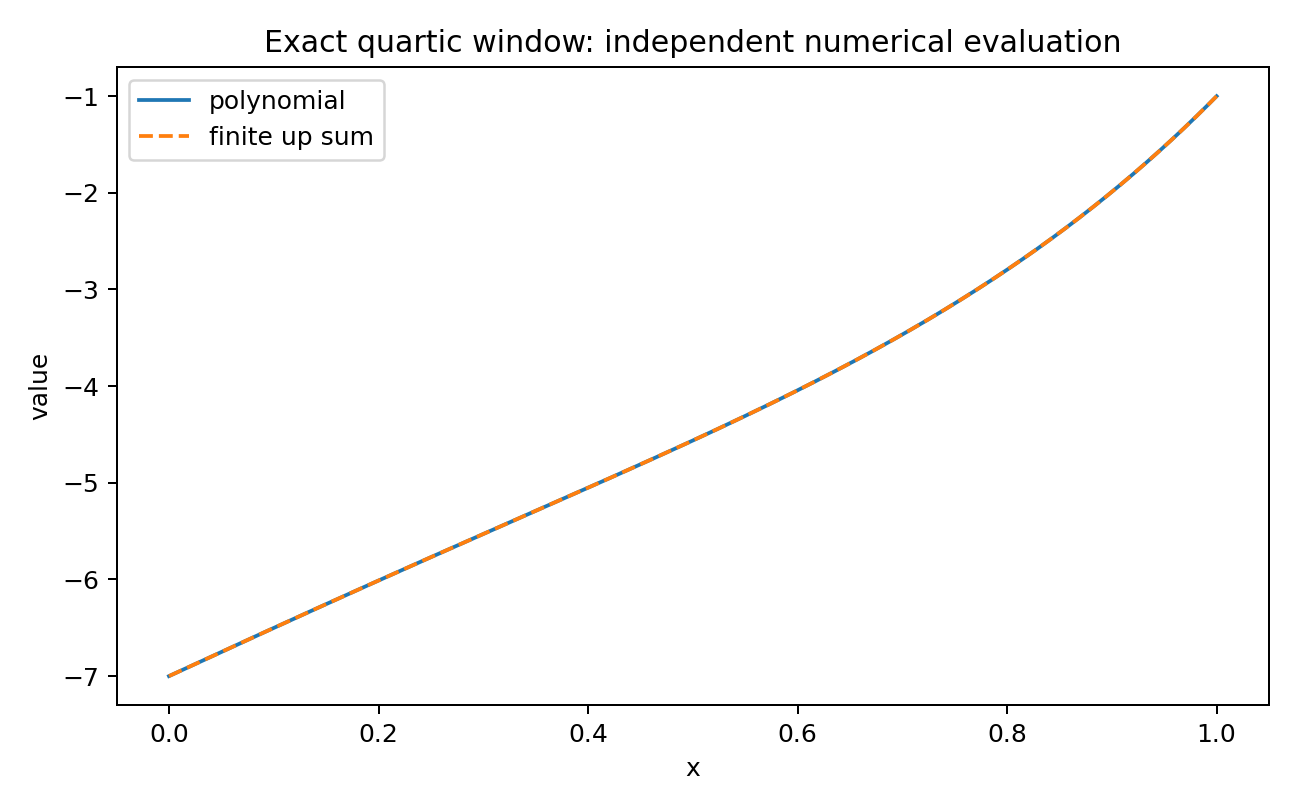
\includegraphics[width=0.72\textwidth]{quartic_reconstruction.png}\\[0.4em]
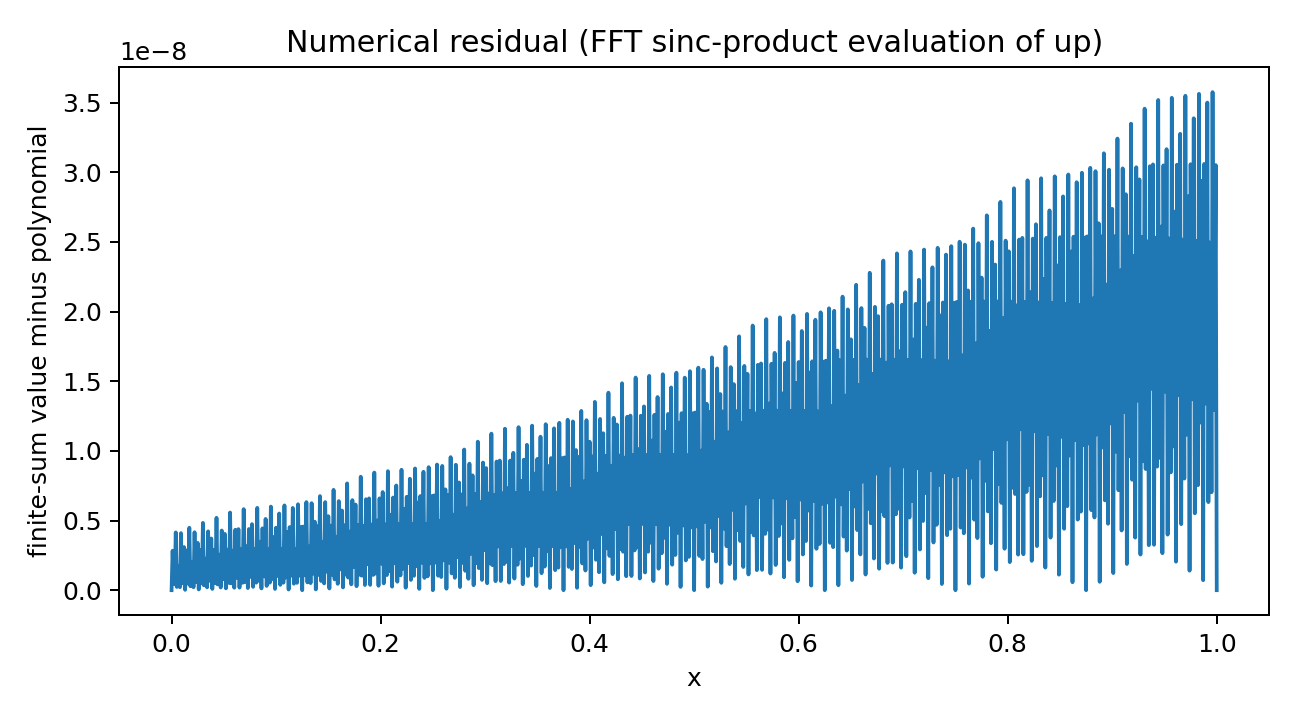
\includegraphics[width=0.72\textwidth]{quartic_residual.png}
\caption{The worked quartic \eqref{eq:quartic}: the ten-atom window
(top, visually indistinguishable from the polynomial on $[0,1]$) and
the residual of the independent FFT check (bottom); the exact
symbolic residual is zero.}
\label{fig:quartic}
\end{figure}

\subsection{Structure: Chebyshev system, extension operator,
collars}

\begin{proposition}[Derivative ladder, Wronskian, interpolation]
\label{prop:ladder-structure}
On $[a,b]$,
$\Psi_{n,h}^{(k)}=\fall nk\,h^{-k}\,\Psi_{n-k,h}$; the Wronskian is
constant,
$W(\Psi_{0,h},\dots,\Psi_{d,h})=h^{-d(d+1)/2}\prod_{n\le d}n!$; and
for distinct nodes $x_0,\dots,x_d\in[a,b]$,
\begin{equation}
 \det\bigl[\Psi_{j,h}(x_i)\bigr]
 =h^{-d(d+1)/2}\prod_{i<j}(x_j-x_i).
 \label{eq:interp-det}
\end{equation}
The block family is thus an extended complete Chebyshev system on
every subinterval, nonsingular for interpolation at every node set.
\end{proposition}

\begin{proof}
On the interval the blocks \emph{are} the monic polynomials
$G_n((x-a+h)/h)$; a monic triangular change of basis has determinant
one, the monomial Wronskian is $\prod n!$, each derivative row scales
by $h^{-k}$, and the interpolation determinant is the Vandermonde in
$y_i=(x_i-a+h)/h$.
\end{proof}

\begin{proposition}[Extension operator and support]
\label{prop:extension}
The map $E_{d,a,b,h}\colon p\mapsto\sum_{n,N}\alpha_{n,N}(p)\,
u\bigl((x-C_{n,N})/2^{n+1}h\bigr)$, with centers
$C_{n,N}=a+h(2^{n+1}-2+2N)$, is a linear injection
$\PiD\to C_c^\infty(\R)$ that restricts to the identity on
$[a,b]$ --- an explicit compactly supported smooth extension operator
for polynomial data, flat at its outer support endpoints, with
\begin{equation}
 \supp E_{d,a,b,h}\,p\subseteq
 \bigl[a-2h,\;a+h(2^{d+2}-2+2K)\bigr]
 \subset\bigl[a-2h,\;b+2^{d+2}h\bigr).
 \label{eq:support}
\end{equation}
\end{proposition}

\begin{theorem}[Collar--atom tradeoff]
\label{thm:collar}
For any collar $\rho>0$, the choice $h=\rho/2^{d+2}$ gives an exact
window supported in $[a-\rho,\,b+\rho]$ with at most
$(d+1)\bigl(1+\ceil{2^{d+1}L/\rho}\bigr)$ atoms.  Conversely the
sparse $h=L/2$ choice has linear atom count $2d+2$ but an
exponentially long one-sided scale ladder,
$\supp\subseteq[a-L,\;a+2^{d+1}L]$.  A reflected anticausal train
(right-tail integration $J_+$) mirrors the overhang, and orientations
may be mixed degree by degree, since any sequence of monic
degree-$n$ blocks remains a triangular basis.
\end{theorem}

\begin{proof}
$2h=\rho/2^{d+1}\le\rho$ bounds the left overhang and
\eqref{eq:support} the right one; the count is
$(d+1)(K+1)$.  The reflection statement is
$J_+u(x)=\sum_{k\ge0}u\bigl(\tfrac{x+2k+1}2\bigr)$ by evenness.
\end{proof}

\begin{remark}[Conditioning]
The level normalization $n!\,2^{n(n+1)/2}$ grows superexponentially
and the paired atoms are sampled near flat support edges, so the
polynomial emerges from cancellation among large terms: construct
coefficients exactly, evaluate in extended precision, sum blockwise
with compensation.  The quasipolynomial law
\eqref{eq:pm-asymptotic} shows why shrinking $h$ does not uniformly
worsen coefficients (normalized weights grow like $N^{n}$ while the
Appell coordinates carry powers of $h$): a nontrivial
conditioning-optimal $h$ should exist
(\cref{conj:conditioning-scale}).  The same warning applies to the
endpoint basis of \cref{sec:dictionary}, whose minimal atom count
also comes at the price of large signed coefficients.
\end{remark}


\section{The oversampled lattice: free scales, ghost antiderivatives,
and the Thue--Morse stencil}
\label{sec:lattice}

The third absorbed source detaches the dictionary construction from
the special lattice $M=2^{d}$ at unit spacing: the reproduction order
depends only on the \emph{ratio} of atom radius to center spacing,
and the physical scale is free.  This adds an interval algorithm with
prescribed support, a real-space antiderivative calculus dual to the
ladder of \cref{sec:ladder}, and the exact dyadic derivative stencil.

\subsection{Twisted Poisson summation and general ratios}

\begin{lemma}[Twisted Poisson identity]
\label{lem:twisted-poisson}
For $m\in\N_{>0}$, $t\in\R$, $z\in\C$, with
$\MM_u$ the moment generating function,
\begin{equation}
 \sum_{k\in\Z}\e^{kz}\,u\!\left(\frac{t-k}{m}\right)
 =m\sum_{n\in\Z}\e^{(z-2\pi\ii n)t}\,
 \MM_u\!\bigl(-mz+2\pi\ii mn\bigr),
 \label{eq:twisted-poisson}
\end{equation}
both sides entire in $z$.
\end{lemma}

\begin{proof}
Poisson summation for the smooth compactly supported
$x\mapsto\e^{zx}u((t-x)/m)$, whose $n$-th Fourier coefficient is
$m\,\e^{(z-2\pi\ii n)t}\MM_u(-mz+2\pi\ii mn)$.
\end{proof}

At a nonzero frequency $n$, the alias factor vanishes at $z=0$ to
order $1+\vtwo(mn)\ge\vtwo(m)+1$.  Dividing
\eqref{eq:twisted-poisson} by $m\MM_u(mz)$ and comparing Taylor
coefficients gives, in one stroke, the general-ratio version of the
global synthesis: with the scaled deconvolution Appell samples
\begin{equation}
 A^{(m)}_r(k):=m^{\,r-1}\,\Gd_r(k/m)
 =\frac1m\sum_{j=0}^{r}\binom rj k^{\,r-j}\,\beta^{(m)}_j,
 \qquad
 \frac1{\MM_u(mz)}=\sum_n\beta^{(m)}_n\frac{z^{n}}{n!},
 \label{eq:scaled-appell}
\end{equation}
one has, for every $m\in\N_{>0}$ and $0\le r\le\vtwo(m)$,
\begin{equation}
 t^{\,r}=\sum_{k\in\Z}A^{(m)}_r(k)\,
 u\!\left(\frac{t-k}{m}\right)
 \qquad(t\in\R),
 \label{eq:general-reproduction}
\end{equation}
locally finite, and the order $\vtwo(m)$ is \emph{sharp}
(\cref{thm:scale-classification}); the same argument works for any
$C_c^\infty$ generator of unit mass whose transform vanishes to
order $d+1$ at the nonzero dual lattice.  The probabilistic content
of the deconvolution is exact:
$q^{\sharp}=\MM_u(mD)^{-1}q$ is the unique polynomial with
$\E\,q^{\sharp}(t+mZ)=q(t)$ --- the coefficients undo smoothing by a
random up-distributed displacement.

The first failure at degree $L=\vtwo(m)+1$ generalizes the defect
series \eqref{eq:defect-series} beyond dyadic ratios: for
$m=2^{\nu}q$ with $q$ odd,
\begin{equation}
 \sum_{k\in\Z}A^{(m)}_L(k)\,u\!\left(\frac{t-k}{m}\right)-t^{L}
 =\frac{(-1)^{L+1}L!}{(2\pi\ii)^{L}}
 \sum_{\substack{n\in\Z\\ n\ \mathrm{odd}}}
 \frac{\widehat u(qn/2)}{n^{L}}\,\e^{-2\pi\ii nt},
 \label{eq:general-defect}
\end{equation}
nonzero because $\widehat u(q/2)\ne0$: an odd factor $q$ in the ratio
replaces the half-integer values $\widehat u(n/2)$ by
$\widehat u(qn/2)$ --- the arithmetic face of the odd-overscaling
phenomenon of \cref{conj:odd-dim}.

\subsection{The physical-scale interval algorithm}

Affine reduction makes the lattice fully physical: for
$p\in\PiD$, an interval $I=[A,B]$, an origin $x_0$, a spacing $h>0$,
and any ratio $m$ with $\vtwo(m)\ge d$ (canonically $m=2^{d}$), put
$\rho=mh$ and
$p^{\sharp}_\rho=\MM_u(\rho D)^{-1}p$.  Then
\begin{equation}
 \boxed{\;
 p(x)=\frac1m
 \sum_{k=\ceil{(A-x_0)/h-m}}^{\floor{(B-x_0)/h+m}}
 p^{\sharp}_\rho(x_0+kh)\,
 u\!\left(\frac{x-x_0-kh}{\rho}\right)
 \qquad(x\in[A,B]),
 \;}
 \label{eq:interval-algorithm}
\end{equation}
a finite $C^\infty$ plateau supported in $[A-2\rho,\,B+2\rho]$ with
at most $\floor{m((B-A)/\rho+2)}+1$ atoms, rational for rational
data, matching \emph{every} endpoint jet of $p$ (all derivatives
agree on the interior; take one-sided limits).  Two practical
features distinguish it from both normal forms above: the
representation is determined by $\bigO(d)$ field elements (the
polynomial $p^{\sharp}_\rho$ and the lattice parameters), however
long the interval; and evaluation at a point touches at most
$2m+1$ atoms.  The atom count
$2^{d}(B-A)/\rho+2^{d+1}+\bigO(1)$ exposes the radius--density
tradeoff: shrinking the support collar costs interior atoms, and the
$2^{d+1}$ boundary-overlap term never disappears --- the lattice-side
counterpart of the ladder's collar--atom law
(\cref{thm:collar}), with the dictionary's $d+2$ and the ladder's
$2d+2$ as the atom-minimal and scale-sparse extremes.

\subsection{Ghost antiderivatives and the exact derivative stencil}

The refinement derivative also supports a purely real-space route,
dual to the antiderivative train of \cref{sec:ladder}.  Writing
$U_{a,c}(x)=u((x-c)/a)$, the \emph{parent--child identity}
\begin{equation}
 D\,U_{2a,c}
 =\frac1a\bigl(U_{a,c-a}-U_{a,c+a}\bigr)
 \label{eq:parent-child}
\end{equation}
converts differentiation into a two-term difference one scale down.
A finite child sum $\sum_{j=L}^{R}b_jU_{a,c+(2j+1)a}$ has a finite
parent antiderivative iff $\sum_jb_j=0$, in which case the parent
coefficients are the prefix sums $\sum_{r\le j}b_r$ --- and the
zero-sum obstruction is repaired by \emph{ghost atoms}: children
whose supports miss the working interval carry the compensating
mass, and the split of that mass between the two ends is a free
constant of integration, canonically fixed by the
$\ell^{2}$- or $\ell^\infty$-optimal choices
$\gamma_2=-\frac1N\sum P_j$,
$\gamma_\infty=-\tfrac12(\max P_j+\min P_j)$.  Iterating from a
partition-of-unity representation of $p^{(d)}$ downward gives a
local, sparse, boundary-adaptable alternative to
\eqref{eq:interval-algorithm} in which scales may change per stage.

Iterating \eqref{eq:parent-child} upward instead gives the exact
dyadic derivative stencil:
\begin{equation}
 \boxed{\;
 D^{\,d}\,U_{2^{d}h,\,c}(x)
 =h^{-d}\,2^{-\binom d2}
 \sum_{k=0}^{2^{d}-1}\eps_k\,
 U_{h,\;c+(2k-(2^{d}-1))h}(x),
 \;}
 \label{eq:tm-stencil}
\end{equation}
with the signed Thue--Morse signs $\eps_k$: each differentiation
doubles the leaves and appends a binary digit carrying the sign, the
chain-rule factors multiplying to $h^{-d}2^{-\binom d2}$.  Together
with \cref{thm:iterated-J} this closes a perfect duality:
\emph{integration} spreads one atom into a train weighted by the
partition numbers $p_m(N)$ (the causal inverse of the Thue--Morse
block, \cref{prop:tm-green}), while \emph{differentiation} contracts
a coarse atom into a block weighted by the Thue--Morse signs
themselves --- the two convolution inverses of one stencil, realized
by up-atoms at dyadic scales.  The Gaussian-binomial deformation
$\prod_{j<d}(1-yq^{j})
=\sum_r(-1)^{r}q^{\binom r2}\genfrac{[}{]}{0pt}{}{d}{r}_q y^{r}$
suggests geometrically scaled stencils
(\cref{q:qgeometric}).

\subsection{Finite sinc prefixes}

Truncating the Fourier product at $N$ factors gives the
piecewise-polynomial generator $u_N$ (an $N$-fold uniform
convolution, support radius $1-2^{-N}$), whose lattice has exact
reproduction degree $\min(N-1,\vtwo(m))$, whose cumulants obey the
exact truncation law
$\kappa^{(N)}_{2r}=(1-2^{-2rN})\,\kappa_{2r}$, and whose Appell
coefficients converge to the up-versions at the dyadic rate
\begin{equation}
 A^{(m)}_{r,N}=A^{(m)}_r
 +\binom r2\kappa_2m^{2}\,2^{-2N}A^{(m)}_{r-2}
 +\bigO_{r,m}\bigl(2^{-4N}\bigr):
 \label{eq:finite-appell}
\end{equation}
exact spline plateaux of any prescribed finite order, converging
coefficientwise to the $C^\infty$ theory.  (The eighth-wave report
absorbed into the exponents volume as its Part~III develops the
prefix generators themselves in depth: an exact truncated-power
formula with Thue--Morse top-derivative jumps, the exact uniform
error law $\lVert u_N-u\rVert_\infty=\tfrac{4}{9}4^{-N}$ with all
derivative orders, and positive quadrature tail surrogates of
arbitrary order.)

\subsection{Verification and arithmetic}

The absorbed package verifies the interval algorithm in exact
rational arithmetic: the worked degree-four example
($p=\tfrac75-3x+2x^{2}-\tfrac12x^{3}+\tfrac37x^{4}$ on
$[-\tfrac12,\tfrac32]$, $m=16$, $\rho=2$,
$p^{\sharp}_2=\tfrac{1301}{1575}-\tfrac73y+\tfrac67y^{2}
-\tfrac12y^{3}+\tfrac37y^{4}$, $49$ atoms) has residual
\emph{exactly zero} at $129$ dyadic points, and seven generic tests
of degrees $0$--$6$ likewise return exact zero
(\nolinkurl{assets/Rvachev_Up_Exact_Polynomial_Representation_Report/}).
Arithmetically, every reduced cumulant $\kappa_{2r}$ has \emph{odd}
denominator (the single factor of two in the reduced denominator of
$B_{2r}$ cancels against $2^{2r-1}/r$), which yields explicit
$2$-adic denominator bounds for all output coefficients: for data in
$2^{-s}\Z[1/O]$ ($O$ odd) the coefficients lie in
$2^{-[s(d+1)+d+\nu]}\Z[1/O']$, all further growth odd
(\cref{q:odd-denominator}).

\section{Dictionary versus ladder, and the minimal atom count}
\label{sec:comparison}

The two constructions solve the same problem with complementary
economies:

\begin{center}
\small
\begin{tabularx}{\textwidth}{@{}p{0.27\textwidth}XX@{}}
\toprule
 & Common-scale dictionary (\cref{sec:dictionary})
 & Scale ladder (\cref{sec:ladder})\\
\midrule
Scales used & one: $2^{d}h$ & $d+1$: $2h,4h,\dots,2^{d+1}h$\\
Atoms for $\PiD$, one cell & $d+2$ (optimal for fixed dictionaries)
 & $2d+2$ (two per degree, equal amplitudes per block)\\
Coefficients & recurrence residual / $H_d(D)$ symbol,
 $\bigO(d^{2})$ & triangular Appell transform, $\bigO(d^{2})$\\
Uniqueness & unique in the endpoint basis
 & unique in the block basis\\
Support overhang & $[a-(d+1)h,\;b+(2M-1)h]$, knob $J$
 & collar $\rho$ at will via $h=\rho/2^{d+2}$, knob $h$\\
Certificate / defect & one-scalar Thue--Morse test; explicit
 $\mathcal D_d$ & exactness by construction (blocks \emph{are}
 $G_n$)\\
Discrete engine & alias annihilator $A_d=\prod[2^{m}]_z$
 & Green inverse $1/\ThetaTM_{m}$, weights $p_m(N)$\\
\bottomrule
\end{tabularx}
\end{center}

The two discrete engines are the two directions of one convolution
identity ($\ThetaTM$ against its causal inverse), and the two
coefficient calculi are the two members of the Appell pair
\eqref{eq:appell-pair}.  The oversampled lattice of
\cref{sec:lattice} is the third normal form, extremal in a third
sense: many atoms ($2^{d}(B-A)/\rho+2^{d+1}+\bigO(1)$) but an
$\bigO(d)$-element \emph{description} with $2m+1$-local
evaluation, a free physical scale, and full endpoint-jet matching
--- with the ghost-antiderivative route as its sparse, per-stage
adaptable variant.  The comparison also settles more of the
minimal-atom question than any source alone.

\begin{theorem}[Minimal atom counts]
\label{thm:minimal-atoms}
Let $N_d$ be the least integer such that \emph{every} real polynomial
of degree at most $d$ admits a representation
\eqref{eq:general-problem} on every nondegenerate interval with at
most $N_d$ atoms.  Then
\begin{equation}
 N_0=2,
 \qquad
 \boxed{\;N_d\le d+2\;}
 \quad(d\ge0),
 \label{eq:Nd-bounds}
\end{equation}
the upper bound achieved by the single fixed endpoint dictionary of
\cref{thm:endpoint-basis}; and every \emph{fixed} dictionary whose
span contains $\PiD$ has at least $d+2$ atoms
(\cref{prop:fixed-lower}).
\end{theorem}

\begin{proof}
$N_0\ge2$ is the strict monotonicity of \cref{sec:problem};
$N_0\le2$ is the partition \eqref{eq:partition-interval}.  For
general $d$ the endpoint basis represents every $P\in\PiD$ with the
same $d+2$ atoms.
\end{proof}

The bound $N_d\le d+2$ sharpens the ladder count $2d+2$ of
\cref{cor:two-atom} --- one of the dividends of consolidating the two
sources.  What remains open is whether \emph{adaptivity} can beat the
dictionary:

\begin{conjecture}[Target-adaptive rigidity]
\label{conj:adaptive-rigidity}
For Lebesgue-almost every $P\in\PiD$ there is no identity
\eqref{eq:general-problem} with $N\le d+1$ atoms, even when
amplitudes, shifts, and scales all depend on $P$; hence
$N_d=d+2$.  The fixed-dictionary case is
\cref{prop:fixed-lower}; the adaptive case replaces a finite union of
proper subspaces by an uncountable parametrized family and appears to
require a rigidity theorem for cancellation among nonanalytic affine
copies of $u$.  Within the causal-ladder class (degree-independent
left support edge, exact degree-$n$ polynomial tails), at least two
atoms per active level are conjectured necessary for generic targets,
making $2d+2$ minimal \emph{in that class}.
\end{conjecture}

\begin{remark}[Strang--Fix reconciliation]
There is no tension with the classical no-go: a single fixed-scale
integer-shift $u$-system reproduces only constants globally
(\cref{thm:scale-classification} at $\vtwo(\rho)=0$).  Both
constructions bypass it lawfully --- the dictionary by paying scale
($\rho=2^{d}$ restores order $d$ globally before localizing), the
ladder by paying scales \emph{and} asking only for a window (boundary
truncation on a bounded interval).  The classical $UP_n$ polynomial
inclusions of Rvachev theory \cite{RvachevRvachev1972,Rvachev1990}
are thereby made explicit in two normal forms.
\end{remark}

\section{Extensions}
\label{sec:extensions}

\subsection{Odd overscaling}
For $\rho=2^{d}q$ with $q$ odd, reproduction order stays $d$
(\cref{thm:scale-classification}) while the alias argument yields the
larger annihilator
$A_{\rho,d}(z)=\prod_{r=0}^{d}\bigl(z^{\rho/2^{r}}-1\bigr)/(z-1)$ of
degree $2\rho-q-d-1$, from the coset multiplicities
$1+\min\{\vtwo(j),d\}$; the one-cell dimension is
$\le q+d+1$, conjecturally with equality
(\cref{conj:odd-dim}): each odd factor buys $q-1$ extra
\emph{defect} directions and no polynomial order.

\subsection{Tensor products and multivariate compression}
On a box in $\R^{s}$, both constructions tensorize: coordinatewise
degrees $(d_1,\dots,d_s)$ cost $\prod_j(d_j+2)$ dictionary atoms or
$\prod_j2(d_j+1)$ ladder atoms, exactly on the tensor polynomial
space.  For \emph{total} degree $d$ the tensor counts far exceed
$\binom{d+s}s$; a multivariate alias-ideal compression (the analogue
of \cref{thm:alias-family} for $\Z^{s}$-cosets) is an attractive
frontier problem.

\subsection{Hermite jet stitching and analytic data}
The derivative ladder of \cref{prop:ladder-structure} exposes all
endpoint jets of the blocks, so finite Hermite systems stitch
different polynomial plateaus on disjoint intervals into one
compactly supported $C^\infty$ function with automatic smooth
transitions --- an atomic-function analogue of splines with
infinitely smooth knots.  For $f$ analytic near $[a,b]$, truncating
the Appell expansion of $f(c+hy)$ at degree $d$ converts any
polynomial-approximation remainder into a finite-atom approximation
bound: the exact theory doubles as a constructive approximation
scheme.

\subsection{Base $b$ and $q$-ary ladders}
Both engines are dyadic only through the zero set of
$\widehat u$.  For an integer base $b\ge2$, the compactly supported
density with transform $\prod_{j\ge0}\sincpi(\xi/b^{j})$ supports the
same two constructions --- dictionary scale $b^{d}$, and ladders
weighted by $b$-ary restricted partition numbers
$[z^{N}]\prod_{j<m}(1-z^{b^{j}})^{-1}$ whenever the derivative
refinement has an integral translation stencil --- with a generalized
Prouhet digit character as certificate.  The dyadic case is the most
arithmetic because the reciprocal stencil is the Thue--Morse block.

\subsection{Positive synthesis and dual functionals}
Sign-changing polynomials force signed amplitudes, but for strictly
positive targets, nonnegative-amplitude synthesis in an overcomplete
dictionary is a finite-dimensional cone-membership problem after
fixing scale and interval (\cref{q:positive}).  Compactly supported
dual functionals $\lambda_n$ with
$\lambda_n(\Psi_m)=\delta_{nm}$ --- ideally finite dyadic samples or
moments of $u$ --- would upgrade the block basis to a local
projection and quadrature calculus (\cref{prob:duals}).

\section{Conjectures, problems, and the Lean program}
\label{sec:frontiers-poly}

Besides \cref{conj:adaptive-rigidity} and
\cref{q:defect-values}:

\begin{conjecture}[Central consecutive basis]
\label{conj:central-basis}
The consecutive central block
$\{\psi_0,\dots,\psi_{d+1}\}|_{[0,1]}$ is a basis of $V_d$ for every
$d$; equivalently the integer determinant
$\Delta^{\mathrm{cen}}_d$ of its reduction to the endpoint basis is
nonzero.  Exact values through $d=12$ support this:
\[
 1,\;1,\;3,\;-1,\;255,\;-6145,\;524287,\;-62914561,\;
 17716740095,\;-9620726743041,
\]
\[
 11047892835893247,\;-25076042725198921729,\;
 113484369541461161541631,
\]
a sequence with visibly rich divisibility (note
$255=2^{8}-1$, $524287=2^{19}-1$) inviting a product, resultant, or
cyclotomic interpretation (\cref{q:central-det}).  Nonvanishing is an
algebraic claim only; some central coordinates are \emph{worse}
conditioned than endpoint ones.
\end{conjecture}

\begin{conjecture}[Odd overscaling dimension]
\label{conj:odd-dim}
For $\rho=2^{d}q$, $q$ odd, the one-cell local space has dimension
exactly $q+d+1$.
\end{conjecture}

\begin{conjecture}[Bit growth]
\label{conj:bit-growth}
The lowest-terms numerators and denominators of the endpoint
coefficients of $t^{d}$ have bit length $\bigO(d^{2})$.  (Plausible
since $\log A_d(1)=\Theta(d^{2})$ and all operator series are
Bernoulli-rational; cancellation makes a proof nontrivial.)
\end{conjecture}

\begin{conjecture}[Support--atom Pareto optimality]
\label{conj:pareto}
For fixed $d$ and collar ratio $\rho/L\to0$, any causal
positive-scale construction with uniformly controlled block condition
numbers needs $\Omega_d(L/\rho)$ atoms; the bound of
\cref{thm:collar} is optimal up to a degree-dependent constant.
\end{conjecture}

\begin{conjecture}[Conditioning-optimal scale]
\label{conj:conditioning-scale}
Natural coefficient and evaluation condition functionals of the
ladder have a finite minimizer in $h>0$, unique up to a short list of
adjacent $K$-regimes.
\end{conjecture}

\begin{question}[Condition-optimal $(d{+}2)$-basis]
\label{q:condition-basis}
Among all $(d+2)$-subsets of the active dyadic dictionary, which
basis minimizes a chosen stability functional ($L^\infty$ coefficient
norm over unit-norm targets, smallest sampled singular value,
Lebesgue-type constant, support overhang)?
\end{question}

\begin{question}[Central determinant sequence]
\label{q:central-det}
Find a recurrence, product formula, or resultant interpretation for
$\Delta^{\mathrm{cen}}_d$ and explain its Mersenne-type prime
content.
\end{question}

\begin{question}[Positive synthesis]
\label{q:positive}
Characterize the polynomials representable with nonnegative
amplitudes in an overcomplete up-dictionary.
\end{question}

\begin{problem}[Dual functionals]
\label{prob:duals}
Construct compactly supported duals of the block (or endpoint) basis
from finite dyadic samples or moments of $u$, and derive the induced
local projection and quadrature formulas.
\end{problem}

\begin{problem}[Weight arithmetic]
\label{prob:weight-arithmetic}
Expand $p_m(N)$ and the normalized monic weights in bases adapted to
Gaussian $q$-binomial coefficients and Prouhet cancellation; make the
lower-order quasipolynomial coefficients explicit as Bernoulli
polynomials on residue classes modulo $2^{m-1}$, and connect them to
Mahler-type functional equations.
\end{problem}

\begin{conjecture}[Lattice minimality and atom complexity]
\label{conj:lattice-minimality}
(i) There is a length threshold $L_d$ such that any exact one-scale
lattice representation of a degree-$d$ polynomial on an interval of
length $\ge L_dh$, with no atom identically zero there, forces
$\vtwo(m)\ge d$: long plateaux cannot beat the stationary binary
order by boundary engineering.  (ii) For intervals comparable to the
atom radius and bounded support enlargement, every one-scale exact
representation of all of $\PiD$ needs $\Omega(2^{d})$ atoms in the
worst case, making the canonical $2^{d+1}+\bigO(1)$ boundary count
order-optimal.  (The fixed-dictionary count of
\cref{prop:fixed-lower} bounds \emph{dimension}; these bound
\emph{lattice atom numbers}.)
\end{conjecture}

\begin{conjecture}[Stable radius, ghost limit, local Chebyshev]
\label{conj:lattice-analytic}
For fixed $p$ and interval, the coefficient norm of the canonical
lattice representation has a finite minimizing radius $\rho_*>0$,
governed by the nearest complex critical scale of
$1/\MM_u(\rho z)$ (the lattice sibling of
\cref{conj:conditioning-scale}).  The $\ell^{2}$-optimal
ghost-antiderivative iterates converge, after matching scale and
lattice, to the canonical Appell samples.  And for generic ordered
centers on a sufficiently short interval avoiding support endpoints,
finite equal-scale up-translate families form an extended Chebyshev
system.
\end{conjecture}

\begin{question}[Sharp odd-denominator law]
\label{q:odd-denominator}
Every reduced cumulant $\kappa_{2r}$ has odd denominator
(\cref{sec:lattice}); determine the exact $2$-adic valuation of the
reduced $A^{(m)}_r(u)$ at dyadic $u$ (conjecturally a function only
of the dyadic denominator of $u$ and the binary digit sums of the
Bell partitions of $r$, all irregular growth confined to odd primes
dividing $2^{2j}-1$ and Bernoulli numerators).
\end{question}

\begin{question}[Endpoint asymptotics of the Appell table]
\label{q:appell-endpoint}
In the boundary scaling $u=1+\delta_d$ with
$\delta_d2^{d}/d$ bounded away from $0$ and $\infty$, the dominant
saddle $z_d$ of $\Gd_d(u)=[z^{d}]d!\,\e^{uz}/\MM_u(z)$ should obey
$d=\delta_dz_d+\log_2z_d+\Theta(1)$, and the full expansion should
carry a nonconstant one-periodic lower-Lambert phase --- the
polynomial-synthesis face of the corpus's Fabius endpoint machinery
(fixed-$u$ coefficients are instead governed by the nearest
imaginary poles of $1/\MM_u$).
\end{question}

\begin{question}[$q$-geometric stencils]
\label{q:qgeometric}
Is there a nonstationary atomic family with geometrically varying
scales whose exact derivative/reproduction stencils have Gaussian
binomial coefficients $(-1)^{r}q^{\binom r2}
\genfrac{[}{]}{0pt}{}{d}{r}_q$, interacting at $q=2$ with the
Rvachev refinement equation and degenerating at $q\to1$ to ordinary
finite differences?  (This subsumes the base-$b$ question of
\cref{sec:extensions} on the stencil side.)
\end{question}

\begin{statusbox}{Lean formalization roadmap}
In dependency order, all finite or formal-power-series layers first:
(1) the telescoping identity of \cref{prop:one-step} and the
binary-partition induction \eqref{eq:iterated-J};
(2) support bookkeeping and the truncation theorem
\cref{thm:finite-window}; (3) finite-dimensional Appell inversion
(\cref{thm:coefficient-transform});
(4) polynomial-weighted Poisson summation and the global synthesis
\cref{thm:global-synthesis} (the analytic core, using the already
formalized integer zero orders);
(5) root-of-unity comb derivatives and the alias multiplicities of
\cref{thm:alias-family}; (6) the $q$-integer factorization
\eqref{eq:A-cyclotomic}; (7) the dimension argument of
\cref{thm:local-dim} via the existing non-elementarity theorem;
(8) recurrence elimination, the Thue--Morse certificate, and the
formal cancellation proof of the $H_d$ symbol
\eqref{eq:H-def}; (9) twisted Poisson summation
\eqref{eq:twisted-poisson} and the general-ratio reproduction
\eqref{eq:general-reproduction}; (10) the parent--child identity,
finite prefix-sum primitive, and the Thue--Morse stencil
\eqref{eq:tm-stencil} (pure finite algebra plus support
reasoning).  Steps (1)--(3), (5)--(8), and (10) are finite
algebra; only (4) and (9) need Schwartz-class Poisson summation.
\emph{Update (28 Aug 2026):} the analytic engine of (4) and (9) is
now largely in the library ---
\nolinkurl{Fabius.tsum_shifted_monomial_eq_integral_real}
(\nolinkurl{MonomialCombExactness.lean}) kernel-verifies the dual
(quadrature) face
$\sum_{k}(\theta+k)^{p}\Up(2^{-m}(\theta+k))
=\int x^{p}\Up(2^{-m}x)\dd x$ for every real shift and $p\le m$,
via Schwartz-class Poisson summation with the nonzero aliases killed
by the integer-zero-order theorem
(\nolinkurl{MonomialCombAlias.lean}); what remains for (4)/(9) is
the Appell-weighted synthesis direction over the same machinery.
\end{statusbox}

\appendix

\section{Low-order operator data}
\label{app:operator-data}

Truncations of the fast symbol (acting on degrees shown):
\[
 H_0=1,\quad H_1=1+\bigO(z^{2}),\quad
 H_2=1-\tfrac5{36}z^{2}+\bigO(z^{4}),
\]
\[
 H_3=1-\tfrac{13}{72}z^{2}+\bigO(z^{4}),\quad
 H_4=1-\tfrac29z^{2}+\tfrac{857}{32400}z^{4}+\bigO(z^{6});
\]
low annihilator coefficients $(a_0,\dots,a_{d+1})$:
$(1,1,0)$, $(1,2,2,2)$, $(1,3,5,7,8)$, $(1,4,9,16,24,32)$,
$(1,5,14,30,54,86,126)$ for $d=1,\dots,5$; and the formula sheet of
the ladder (all objects rational):
\begin{center}
\small
\begin{tabular}{@{}ll@{}}
\toprule
cumulants & $\kappa_{2m}=B_{2m}/(2m(1-4^{-m}))$, odd zero\\
reciprocal MGF & $\gamma_0=1$,\ \
$\gamma_n=-\sum_{r}\binom{n-1}{r-1}\kappa_r\gamma_{n-r}$\\
blocks & $\Psi_{n,h}
=n!2^{n(n+1)/2}\sum_{N\le K}p_{n+1}(N)\,
u\bigl((x-C_{n,N})/2^{n+1}h\bigr)$\\
centers/scales & $C_{n,N}=a+h(2^{n+1}-2+2N)$,\quad $2^{n+1}h$,\quad
$K=\ceil{(b-a)/2h}$\\
coordinates & $b_n=\sum_r\gamma_rh^{n+r}p^{(n+r)}(a-h)/(n!\,r!)$\\
amplitudes & $\alpha_{n,N}=n!2^{n(n+1)/2}b_np_{n+1}(N)$\\
support & $[a-2h,\;a+h(2^{d+2}-2+2K)]$\\
\bottomrule
\end{tabular}
\end{center}

\section{Provenance of the absorbed sources}
\label{sec:provenance-poly}

\begin{center}
\small
\begin{tabular}{@{}p{0.44\textwidth}p{0.50\textwidth}@{}}
\toprule
Source (directory; SHA-256 of main \texttt{.tex}) & Contribution \\
\midrule
\emph{Exact Polynomial Synthesis by Finite Rvachev Up-Function
Dictionaries}
(\nolinkurl{Rvachev_Up_Polynomial_Representation_Package};
\texttt{a574b30dadbc\ldots})
& The common-scale construction of
\cref{sec:dictionary,sec:certificate}: scale classification, Poisson
collapse, deconvolution synthesis, alias nullspace and $q$-integer
annihilator, $\dim V_d=d+2$, endpoint basis and fixed-dictionary
minimality, output-sensitive $H_d$ algorithm, multi-cell theorem,
Thue--Morse certificate, canonical defect and Fourier residue,
central-basis determinants, odd overscaling, monomial examples and
exact data files. \\
\addlinespace
\emph{Exact Polynomial Windows from Finite Sums of Shifted and Scaled
Rvachev up Functions}
(\nolinkurl{rvachev_up_polynomial_representation};
\texttt{98fe2e5fd256\ldots})
& The ladder construction of \cref{sec:ladder}: antiderivative train,
binary-partition weights and Thue--Morse Green pair, quasipolynomial
structure, tail polynomials, finite-window and two-atom theorems,
Appell coefficient transform with Bernoulli--Bell closed forms,
Wronskian/Chebyshev structure, extension operator, collar--atom
tradeoff, anticausal mixing, conditioning analysis, worked quartic
with figures, classical Rvachev bibliography. \\
\addlinespace
\emph{Exact Polynomial Plateaux from Rvachev's Up-Function}
(seventh wave;
\nolinkurl{Rvachev_Up_Exact_Polynomial_Representation_Report};
SHA in \nolinkurl{assets/SHA256SUMS-absorbed.txt})
& The oversampled lattice of \cref{sec:lattice}: twisted Poisson
identity, general-ratio reproduction with sharp order
$\vtwo(m)$ and the general first-defect series
\eqref{eq:general-defect}, probabilistic deconvolution
characterization, the physical-scale interval algorithm with
truncation indices, support/atom-count bounds, jet matching,
compressed $\bigO(d)$ description and $(2m+1)$-locality; the
ghost-atom antiderivative calculus and the Thue--Morse derivative
stencil \eqref{eq:tm-stencil}; finite sinc-prefix generators with
the exact cumulant truncation law; generator-independent theorem;
odd-cumulant-denominator arithmetic; worked degree-four example with
exact-zero verification; the lattice-side conjectures and questions
of \cref{sec:frontiers-poly}. \\
\bottomrule
\end{tabular}
\end{center}

The exact SHA-256 hashes of the three absorbed \texttt{.tex} sources
are recorded in \nolinkurl{assets/SHA256SUMS-absorbed.txt}.
\emph{What was deduplicated}: the corpus background (normalization,
probability model, MGF/cumulants, Fourier zeros), the Appell
calculus (the third source's up-Appell family
$A^{(m)}_r(u)=m^{r-1}\Gd_r(u/m)$ is the same deconvolution family in
a scaled normalization --- verified on $P_2,P_4$), the Thue--Morse
products, the sharp-order statement (the third source's exact
stationary order $\vtwo(m)$ is
\cref{thm:scale-classification}), rationality and affine covariance,
tensor products (the third source adds per-coordinate ratios),
extension-operator remarks, conditioning warnings, and the Lean
roadmaps.
\emph{What is new to the consolidation}: the unified Appell-pair and
Green-pair framing of \cref{sec:shared}, the comparison table and the
sharpened bound $N_d\le d+2$ of \cref{thm:minimal-atoms}, and the
cross-volume identities of \cref{sec:defect-crosswalk} --- the
defect--quadrature duality \eqref{eq:defect-duality} with its exact
special values \eqref{eq:defect-values}, cross-validated against the
companion volume's independently computed phase-error table.  Beyond
notation, no mathematical content of either source was discarded.
Both sources audited the repository corpus (67-path inventory) and
agree that the explicit finite constructions were absent from it;
that corpus-relative novelty standard is inherited here.

\begin{thebibliography}{99}

\bibitem{Fabius1966}
J.~Fabius,
\newblock A probabilistic example of a nowhere analytic
$C^\infty$-function,
\newblock \emph{Zeitschrift f\"ur Wahrscheinlichkeitstheorie und
Verwandte Gebiete} \textbf{5} (1966), 173--174.

\bibitem{RvachevRvachev1971}
V.~L.~Rvachev and V.~A.~Rvachev,
\newblock A certain finite function,
\newblock \emph{Dopovidi Akademii Nauk Ukrains'koi RSR, Series A}
(1971), 705--707, 764.

\bibitem{RvachevRvachev1972}
V.~L.~Rvachev and V.~A.~Rvachev,
\newblock On the representation of polynomials by functions with
compact support,
\newblock \emph{Mathematical Physics}, No.~11, Naukova Dumka, Kiev,
1972, 126--129.

\bibitem{Rvachev1977}
V.~A.~Rvachev,
\newblock On approximation by means of the function $\Up(x)$,
\newblock \emph{Doklady Akademii Nauk SSSR} \textbf{233} (1977),
no.~2, 295--296.

\bibitem{Rvachev1990}
V.~A.~Rvachev,
\newblock Compactly supported solutions of functional-differential
equations and their applications,
\newblock \emph{Russian Mathematical Surveys} \textbf{45} (1990),
no.~1, 87--120.

\bibitem{Arias1982}
J.~Arias de Reyna,
\newblock Definici\'on y estudio de una funci\'on indefinidamente
diferenciable de soporte compacto,
\newblock \emph{Rev.\ Real Acad.\ Ciencias Madrid} \textbf{76}
(1982), 21--38; English translation arXiv:\nolinkurl{1702.05442}.

\bibitem{Arias2018}
J.~Arias de Reyna,
\newblock Arithmetic of the Fabius function,
\newblock \emph{INTEGERS} \textbf{18} (2018), Article A51.

\bibitem{StrangFix1973}
G.~Strang and G.~Fix,
\newblock A Fourier analysis of the finite element variational
method,
\newblock in \emph{Constructive Aspects of Functional Analysis},
C.I.M.E., 1973, pp.~793--840.

\bibitem{Jia1998}
R.-Q.~Jia,
\newblock Shift-invariant spaces and linear operator equations,
\newblock \emph{Israel Journal of Mathematics} \textbf{103} (1998),
259--288.

\bibitem{deBoorRon1992}
C.~de~Boor and A.~Ron,
\newblock Fourier analysis of the approximation power of principal
shift-invariant spaces,
\newblock \emph{Constructive Approximation} \textbf{8} (1992),
427--462.

\bibitem{deBoorDeVoreRon1994}
C.~de~Boor, R.~A.~DeVore, and A.~Ron,
\newblock Approximation from shift-invariant subspaces of
$L_2(\R^{d})$,
\newblock \emph{Transactions of the American Mathematical Society}
\textbf{341} (1994), 787--806.

\bibitem{CharinaProtasov2021}
M.~Charina and V.~Yu.~Protasov,
\newblock Analytic functions in local shift-invariant spaces and
analytic limits of level dependent subdivision,
\newblock \emph{Journal of Fourier Analysis and Applications}
\textbf{27} (2021), Article 45.

\bibitem{Lee2009}
S.~L.~Lee,
\newblock Approximation of Gaussian by scaling functions and
biorthogonal scaling polynomials,
\newblock \emph{Bull.\ Malays.\ Math.\ Sci.\ Soc.\ (2)} \textbf{32}
(2009), no.~3, 261--282.

\bibitem{Kravchenko2015}
V.~F.~Kravchenko, O.~V.~Kravchenko, Ya.~Yu.~Konovalov,
V.~I.~Pustovoit, and D.~V.~Churikov,
\newblock Atomic, WA-systems, and R-functions applied in modern radio
physics problems: Part III,
\newblock \emph{Journal of Communications Technology and Electronics}
\textbf{60} (2015), 707--736.

\bibitem{Roman1984}
S.~Roman,
\newblock \emph{The Umbral Calculus},
\newblock Academic Press, 1984.

\bibitem{Andrews1998}
G.~E.~Andrews,
\newblock \emph{The Theory of Partitions},
\newblock Cambridge University Press, 1998 reprint.

\bibitem{Comtet1974}
L.~Comtet,
\newblock \emph{Advanced Combinatorics},
\newblock Reidel, 1974.

\bibitem{AlloucheShallit2003}
J.-P.~Allouche and J.~Shallit,
\newblock \emph{Automatic Sequences: Theory, Applications,
Generalizations},
\newblock Cambridge University Press, 2003.

\bibitem{ProveItPrimary}
V.~Reshetnikov,
\newblock \emph{The Fabius Function and Rvachev's Up-Function},
\newblock primary exposition in the \texttt{ProveIt} repository,
\repo, snapshot 28 August 2026.

\bibitem{ProveItDyadicComb}
V.~Reshetnikov,
\newblock \emph{Dyadic-Comb Frontiers for the Fabius--Rvachev
System},
\newblock consolidated frontier volume,
\nolinkurl{drafts/inverse-and-sampling/Dyadic_Comb_Frontiers/},
28 August 2026.

\bibitem{ProveItInverse}
V.~Reshetnikov,
\newblock \emph{Inverse and Sampling Frontiers for the
Fabius--Rvachev System},
\newblock consolidated frontier volume,
\nolinkurl{drafts/inverse-and-sampling/Inverse_and_Sampling_Frontiers/},
2026.

\end{thebibliography}

\end{document}
